\documentclass{ntmanuscript}
\usepackage[acronym,toc]{glossaries}
\newacronym{MIT}{MIT}{the Massachusettes Institute of Technology}
\newacronym{UW}{UW}{University of Wisconsin}
\newacronym{US}{US}{United States}
\newacronym{IAEA}{IAEA}{International Atomic Energy Agency}
\newacronym{SNF}{SNF}{spent nuclear fuel}
\newacronym{HLW}{HLW}{high level waste}
\newacronym{FEHM}{FEHM}{Finite Element Heat and Mass Transfer}
\newacronym{DOE}{DOE}{Department of Energy}
\newacronym{GENIUSv2}{GENIUS}{Global Evaluation of Nuclear Infrastructure Utilization Scenarios, Version 2}
\newacronym{CNERG}{CNERG}{Computational Nuclear Engineering Research Group}
\newacronym{GDSM}{GDSM}{Generic Disposal System Model}
\newacronym{GDSE}{GDSE}{Generic Disposal Sytem Environment}
\newacronym{GPAM}{GPAM}{Generic Performance Asessment Model}
\newacronym{FEPs}{FEPs}{Features, Events, and Processes}
\newacronym{EBS}{EBS}{Engineered Barrier System}
\newacronym{EDZ}{EDZ}{Excavation Disturbed Zone}
\newacronym{YMR}{YMR}{Yucca Mountain Repository Site}
\newacronym{EPA}{EPA}{Environmental Protection Agency}
\newacronym{PEI}{PEI}{Peak Environmental Impact}
\newacronym{VISION}{VISION}{the Verifiable Fuel Cycle Simulation Model}
\newacronym{NUWASTE}{NUWASTE}{Nuclear Waste Assessment System for Technical Evaluation}
\newacronym{NWTRB}{NWTRB}{Nuclear Waste Technical Review Board}
\newacronym{OCRWM}{OCRWM}{Office of Civillian Radioactive Waste Management}
\newacronym{UFD}{UFD}{Used Fuel Disposition}
\newacronym{DYMOND}{DYMOND}{Dynamic Model of Nuclear Development }
\newacronym{DANESS}{DANESS}{Dynamic Analysis of Nuclear Energy System Strategies}
\newacronym{CAFCA}{CAFCA}{ Code for Advanced Fuel Cycles Assessment }
\newacronym{ORION}{ORION}{O..}
\newacronym{NFCSim}{NFCSim}{Nuclear Fuel Cycle Simulator}
\newacronym{COSI}{COSI}{Commelini-Sicard}
\newacronym{FCT}{FCT}{Fuel Cycle Technology}
\newacronym{SWF}{SWF}{Separations and Waste Forms}
\newacronym{FCO}{FCO}{Fuel Cycle Options}
\newacronym{RDD}{RD\&D}{Research Development and Design}
\newacronym{WIPP}{WIPP}{Waste Isolation Pilot Plant}
\newacronym{ANDRA}{ANDRA}{Agence Nationale pour la gestion des D\'echets RAdioactifs, the French National Agency for Radioactive Waste Management}
\newacronym{TSM}{TSM}{Total System Model}
\newacronym{LANL}{LANL}{Los Alamos National Laboratory}
\newacronym{INL}{INL}{Idaho National Laboratory}
\newacronym{ANL}{ANL}{Argonne National Laboratory}
\newacronym{SNL}{SNL}{Sandia National Laboratory}
\newacronym{LBNL}{LBNL}{Lawrence Berkeley National Laboratory}
\newacronym{LLNL}{LLNL}{Lawrence Livermore National Laboratory}
\newacronym{NAGRA}{NAGRA}{National Cooperative for the Disposal of Radioactive Waste}
\newacronym{CUBIT}{CUBIT}{CUBIT Geometry and Mesh Generation Toolkit}
\newacronym{CSNF}{CSNF}{Commercial Spent Nuclear Fuel}
\newacronym{DSNF}{DSNF}{DOE Spent Nuclear Fuel}
\newacronym{MTHM}{MTHM}{Metric Ton of Heavy Metal}
\newacronym{HTGR}{HTGR}{High Temperature Gas Reactor}
\newacronym{TRISO}{TRISO}{Tristructural Isotropic}
\newacronym{MA}{MA}{Minor Actinide}
\newacronym{CEA}{CEA}{Commissariat a l'Energie Atomique et aux Energies Alternatives}
\newacronym{SKB}{SKB}{Svensk Karnbranslehantering AB}
\newacronym{SINDAG}{SINDA{\textbackslash}G}{Systems Improved Numerical Differencing Analyzer $\backslash$ Gaski}
%\newacronym{<++>}{<++>}{<++>}

\usepackage{multicol}
\makeglossaries
%%%%%%%%%%%%%%%%%%%%%%%%%%%%%%%%%%%
\title{Key Processes and Parameters in a Generic Clay Disposal System Model}

% Authors. Separated by commas
\author{Kathryn D.~Huff $^1$, W. Mark~Nutt$^2$}

% Institutes of the authors
\institute{$^1$University of California, Department of Nuclear Engineering Berkeley, CA, 94720\\ $^2$Argonne National Laboratory, Nuclear Engineering Division, 60439} 

% Information concerning the person submitting the manuscript
\submitter{Kathryn D.~Huff}
\submitteraddress{540 O'Farrell, Apartment 501, San Francisco, CA 94102}
\submitteremail{katyhuff@gmail.com}

% No more than three keywords, though each can be a phrase
\keywords{radionuclide containment, hydrologic contaminant transport, 
nuclear repository simulation.}

\usepackage{graphicx}
\usepackage{booktabs} % nice rules for tables
\usepackage{microtype} % if using PDF
\newcommand{\units}[1] {\:\text{#1}}%
\newcommand{\SN}{S$_N$}%{S$_\text{N}$}%{$S_N$}%

% Tabularx has small row height :
\setlength{\extrarowheight}{2pt}

\date{}
%%%%%%%%%%%%%%%%%%%%%%%%%%%%%%%%%%%
\begin{document}
\newpage

%%%%%%%%%%%%%%%%%%%%%%%%%%%%%%%%%%%%%%%%%%%%%%%%%%%%%%%%%%%%%%%%%%%%%%%%%%%%%%%%

%\begin{keywords}
%Nuclear fuel cycle, Repository, Hydrologic Contaminant Transport, 
%Clay.
%\end{keywords}
\begin{abstract}

% Every paper must have an abstract.  The abstract must be less than one page 
% long, double-spaced, and in 12-point font size. 

% the importance of these results as new information, 
% and the major conclusions.  

% It must summarize the content of the paper 
Sensitivity analyses identifying key processes and parameters in saturated, 
homogeneous, clay repository environments were performed. 
% and point out the main objectives, 
The parametric relationships described in this work inform the importance of 
repository site and engineered barrier features in the context of fuel cycle 
decisions. This work characterized per-isotope contaminant transport sensitivity 
to geochemical and hydrologic factrs such as solubility, sorption, 
diffusivity, and vertical advective velocity. It also characterized performance 
sensitivity to engineered barrier performance expectations such as waste form 
degradation rate and the time waste package failure. 
% the methods employed, 
Individual and coupled parameter analyses were undertaken within the GoldSim 
simulation software, which tracks the movement of key radionuclides through the 
natural system and engineered barriers. The per-isotope resolution of the 
results inform the potential impacts of fuel cycle decisions on repository 
performance.
% the results obtained
The results here provide an overview of the relative importance of processes 
determining repository performance of a simplified generic disposal concept in 
saturated, homogeneous environments.  Thresholds between primarily diffusive and 
primarily advective transport were identified and the relative influences of 
geological and engineered barrier parameters on the mobility of dose 
contributing isotopes were characterized.  
%  General and well-known information should not be included in the abstract.
\end{abstract}

\newpage

\twocolumn
%%%%%%%%%%%%%%%%%%%%%%%%%%%%%%%%%%%%%%%%%%%%%%%%%%%%%%%%%%%%%%%%%%%%%%%%%%%%%%%%

\section{Introduction}

The development of sustainable nuclear fuel cycles is a key challenge as the use 
of nuclear power expands domestically and internationally. Accordingly, the 
United States and other nations are considering a number of nuclear fuel cycle 
and geologic disposal options simultaneously \cite{}. These decisions are 
technologically coupled since radionuclide containment performance of a geologic 
repository is, in part, a function of spent fuel and high level waste 
composition, which varies among fuel cycle options. Accordingly, integrated 
fuel cycle and disposal system analysis grows increasingly necessary for 
informing spent nuclear fuel management policy.  This work enables that analysis 
by identifying dominant physics of radionuclide and heat transport phenomena 
affecting repository performance in homogeneous, reducing geologic media and as 
a function of spent fuel composition. 
%The long term performance characteristics of deep geologic disposal concepts 
%are affected by heat and radionuclide release characteristics sensitive to 
%disposal system choices as well as variable spent fuel compositions associated 
%with alternative fuel cycles. 

Sensitivity analyses using a detailed multiphysics simulation have characterised 
key performance parameters in a candidate repository concept. This concept 
includes a homogeneous, reducing geologic host media, and limited lifetime 
engineered barrier components.  This sensitivity analysis characterizes the 
sensitivity of repository performance to various site and design parameters in 
the context of competing and coupled physics. Finally, this work informs the 
extent to which fuel cycle decisions, such as separation and transmutation 
strategies, may affect performance.


Previous work in the United States has focused on the oxidizing, fractured 
granite tuff of Yucca Mountain. International work has focused more on reducing 
and homogeneous geologies, but most sensitivity analysis has been site-specific 
\cite{swift/nutt, redimpact}.

Parameters of particular interest in fuel cycle systems analysis have 
historically been those related to the front end of the fuel cycle [citation 
please]. However, parameters representing decisions concerning the back end of 
the fuel cycle are of increasing interest as repositories are being considered 
internationally and as the United States further investigates repository 
alternatives to the Yucca Mountain Repository Site (YMR). Choices such as 
geologic media, engineered barriers, appropriate loading strategies and 
schedules are all independent parameters up for debate. Due to the coupled 
nature of repository capacity and performance, these parameters are coupled with 
decisions about the fuel cycle.  For this reason, sensitivity studies of a 
generic disposal model is necessary to illuminate performance distinctions of 
candidate repository host media, designs, and engineering components in the 
context of varying spent fuel compositions. 

\section{Background}
These analyses were performed using the Clay \gls{GDSM} developed by the 
\gls{UFD} campaign\cite{clayton_generic_2011}. The Clay \gls{GDSM} is built on 
the 
GoldSim software and tracks the movement of key radionuclides through the 
natural system and engineered barriers \cite{golder_goldsim_2010, 
golder_goldsim_ct_2010}.

The disposal concept modeled by the Clay \gls{GDSM} includes an \gls{EBS} which 
can undergo rate based dissolution and barrier failure. Releases from the 
\gls{EBS} enter 
near field and subsequently far field host rock regions in which diffusive and 
advective transport take place, attenuated by solubility limits as well as 
sorption and dispersion phenomena.  

The Clay \gls{GDSM} models a single waste form, a waste package, additional 
\glspl{EBS}, 
an \gls{EDZ}, and a far field zone using a batch reactor mixing cell framework. 
This waste unit cell is modeled 
with boundary conditions such that it may be repeated assuming an infinite 
repository configuration. The waste form and engineered barrier system are 
modeled as well-mixed volumes 
and radial transport away from the cylindrical base case unit cell is modeled as  
one dimensional. Two radionuclide release pathways are considered. One is the 
nominal, 
undisturbed case, while the other is a fast pathway capable of simulating a 
hypothetical disturbed case 
\cite{clayton_generic_2011}.


%%%%%%%%%%%%%%%%%%%%%%%%%%%%%%%%%%%%%%%%%%%%%%%%%%%%%%%%%%%%%%%%%%%%%%%%%%%%%%%%

\section{Description of the Actual Work}

\subsection{Clay Generic Disposal System Model}

% used existing gdsms 
These analyses were performed using the Clay \gls{GDSM} developed by the 
\gls{UFD} campaign \cite{clayton_generic_2011}. 

The Clay \gls{GDSM} is built on the GoldSim simulation framework and contaminant 
transport model.  This radionuclide transport toolset simulates chemical and 
physical attenuation processes including radionuclide solubility, dispersion 
phenomena, and reversible sorption \cite{golder_goldsim_2010, 
golder_goldsim_ct_2010}. Model input parameters supporting modeling of these tranport 
processes include geometry specifications (e.g. repository depth), geologic 
material properties (e.g. clay porosity), geochemical data 
(e.g. elemental solubility limits), and environmental parameters (e.g. natural 
system velocity). Probabilistic elements of the GoldSim modeling 
framework enable the models to incorporate simple probabilistic \gls{FEPs} that 
affect repository performance.

The disposal concept modeled by the Clay \gls{GDSM} is an array of spent nuclear 
fuel packages within a clay repository envrionment, 500 meters beneath the 
earth's surface. In this repository concept, the waste packages contain an 
inventory of spent nuclear fuel, are emplaced horizontally in excavated tunnels, 
and are backfilled by a reducing bentonite clay buffer material within the 
tunnel \cite{nutt_generic_2009}. 

In the \gls{UFD} \gls{GDSM} tool that was used for this analysis, the clay 
repository concept is modeled using a single rectangular disposal cell. The 
disposal cell models a single cylindrical spent nuclear fuel package surrounded 
by bentonite buffer material and emplaced in the clay geologic medium. Using 
reflective boundary conditions in the horizontal plane, an infinite disposal 
cell array is modeled \cite{clayton_generic_2009}.

The model includes vertical advective fast pathway as well as an \gls{EBS} which 
can undergo rate based dissolution and barrier failure.  Releases from the 
\gls{EBS} enter near field and subsequently far field host rock regions in which 
diffusive and advective transport take place, attenuated by solubility limits as 
well as sorption and dispersion phenomena \cite{clayton_generic_2011}.

\subsection{Sampling Scheme}

This analysis has undertaken an analysis strategy to develop a many dimensional 
overview of the key factors in modeled repository performance. To achieve this, 
both individual and dual parametric cases were performed.

Individual parameter cases varied a single parameter of interest in 
detail over a broad range of values. Dual parameter cases were 
performed for pairs of parameters expected to exhibit some covariance. For 
each parameter or pair of parameters, forty simulation 
groups varied the parameter or parameters within the range considered. Each 
case and its parametric range are detailed in Table \ref{tab:Cases}. 

\begin{table}[ht!]
\centering
\footnotesize{
\begin{tabular}{|l|l|l|r|r|}
\multicolumn{5}{c}{\textbf{Simulation Cases}}\\
\hline
\textbf{Case} & \textbf{Parameter} & \textbf{Units} & \textbf{Min. Value} & \textbf{Max. Value}\\
\hline
I     & $D_{eff}$    & $[m^2\cdot s^{-1}]$       & $10^{-8}$    &  $10^{-5}$ \\
      & Inventory              & [MTHM]         & $10^{-4}$    &  $10^1$ \\
\hline
II    & $V_{adv, y}$ & $[m \cdot yr^{-1}]$       & $6.31\times10^{-8}$  &  $6.31\times10^{-4}$ \\
      & $D_{eff}$    & $[m^2\cdot s^{-1}]$       & $10^{-8}$    &  $10^{-5}$ \\
\hline
III   & $S_i$        & $[mol\cdot m^{-3}]$       & $(1\times10^{-9})\langle S_i\rangle $    &  $(5\times10^{10})\langle S_i\rangle $ \\
\hline
IV    & $K_{d,i}$    & $[m^3\cdot kg^{-1}]$       & $(1\times10^{-9})\langle K_{d,i}\rangle $    &  $(5\times10^{10})\langle K_{d,i}\rangle $ \\
\hline
V     & $R_{WFDeg.}$           & $[yr^{-1}]$       & $10^{-9}$    &  $10^{-2}$ \\
      & Inventory              & [MTHM]         & $10^{-4}$    &  $10^1$ \\
\hline 
VI    & $t_{WPFail}$        & $[yr]$         & $10^3$    &  $10^7$ \\
      & $D_{eff}$           & $[m^2\cdot s^{-1}]$       & $10^{-8}$    &  $10^{-5}$ \\
\hline
\end{tabular}
\caption{Each dual and single parameter simulation case had 40 simulation 
groups of 100 realizations each.}
\label{tab:Cases}
}
\end{table}

For each simulation group, a 100 realization simulation was completed. Each
realization held the parameters being analyzed as constant and sampled 
stochastic values for uncertain parameters not being studied.  A sampling scheme 
developed in previous generic disposal media modeling was implemented in this 
model in order to ensure that the each 100 realization simulation sampled 
identical values for uncertain parameters \cite{clayton_generic_2011, 
nutt_generic_2009}.  


\subsection{Mean of the Peak Annual Dose}

In this analysis, repository performance is quantified by radiation dose to a 
hypothetical receptor. Specifically, this sensitivity analysis focuses 
on parameters that affect the mean of the peak annual dose.  The mean of the 
peak annual dose,

\begin{align} \label{MoP}
  D_{MoP,i} &= \frac{\sum_{r=1}^{N}{\max\left[\left.D_{r,i}(t)\right|_{\forall t}\right]}}{N}
  \intertext{where}
  D_{MoP,i} &= \mbox{ mean of peak annual dose due to isotope i } [mrem/yr]\nonumber\\
  D_{r,i}(t) &= \mbox{ year t dose in realization r due to isotope i } [mrem/yr]\nonumber\\
  N &= \mbox{number of realizations, } \nonumber
\end{align}

is a conservative metric of repository performance and should not be confused 
with the peak of the mean annual dose.

%\begin{align} \label{PoM}
%  D_{PoM,i} &= \max\left[{\frac{\sum_{r=1}^{N}{\left.D_{r,i}(t)\right|_{\forall t}}}{N}}\right]\\
%            &= \mbox{peak of the mean annual dose due to isotope i } [mrem/yr].\nonumber
%\end{align}



%%%%%%%%%%%%%%%%%%%%%%%%%%%%%%%%%%%%%%%%%%%%%%%%%%%%%%%%%%%%%%%%%%%%%%%%%%%%%%%%
\section{Clay}

\subsection{Diffusion Coefficient of Far Field}
\label{sec:diffusivity}

In clay media, diffusion dominates far field hydrogeologic transport due to 
characteristically low hydraulic head gradients and permeability. Thus, the 
effective diffusion coefficient, $D_{eff}$, is a parameter to which repository 
performance in clay media is very sensitive. 

The sensitivity of the peak dose to the diffusion coefficient in the 
host rock was analyzed in conjunction with the was inventory total mass. 
to cover the full range of expected diffusion coefficients in clay and 
inventories in current wasteforms.

In order to isolate the effect of the far field behavior, the waste form 
degradation rate was set to be very high as were the solubility and advective 
flow rate through the  \gls{EBS}. This unhindered contaminant flowthrough 
in the near field and left far field transport as the sole remaining physical 
barrier to release.

The peak doses due to highly soluble, non-sorbing elements such as $I$ and $Cl$, 
were found to be proportional to the radionuclide inventory and 
largely directly proportional to the relative diffusivity. In the absence of 
solubility limitation and sorption, the peak dose was shown to be directly 
proportional to mass factor. 

With the exception of those dose-contributors assumed to be completely soluble, 
two regimes were visible in the results of this analysis. In the low diffusion 
coefficient regime, the diffusive pathway through the homogeneous permeable 
porous medium in the far field continues to be a  dominant barrier to nuclide 
release for normal (non-intrusive) repository conditions. 

In the second regime, for very high diffusion coefficients, the effects of 
additional attenuation phenomena in the natural system can be seen.  The 
dependence of peak annual dose on mass factor was consistently directly 
proportional for all isotopic groups.

The peak doses due to solubility limited, sorbing elements such as $Np$ and 
$Tc$ demonstrate two major regimes. In the first regime, for 
low values of mass factor, the mean of the peak annual dose rates is directly 
proportional to both reference diffusivity and mass factor.  For higher values 
of mass factor, the sensitivity to reference diffusivity and mass factor are 
both attenuated at higher values.  The attenuation in these regimes 
is due to natural system attenuation, most notably, sorption.


\begin{frame}[c]
  \frametitle{Case II : Vertical Advective Velocity and Diffusion Coefficient}
Advection is transport driven by bulk water velocity while diffusion is the 
result of Brownian motion across concentration gradients.  The method by which 
the dominant solute transport mode (diffusive or advective) is determined for a 
particular porous medium is by use of the dimensionless Peclet number, 

\begin{align} 
  Pe &= \frac{nvL}{\alpha nv + D_{eff}},\\
  &= \frac{\mbox{advective rate}}{\mbox{diffusive rate}}\nonumber
  \intertext{where} 
  n &= \mbox{ solute accessible porosity } [\%]\nonumber\\
  v &= \mbox{ advective velocity } [m\cdot s^{-1}] \nonumber\\
  L &= \mbox{ transport distance } [m]\nonumber\\
  \alpha &= \mbox{ dispersivity } [m]\nonumber\\
  D_{eff} &= \mbox{ effective diffusion coefficient } [m^2\cdot s^{-1}].\nonumber
\end{align}
For a high $Pe$ number, advection is the dominant transport mode, while 
diffusive or dispersive transport dominates for a low $Pe$ number
\cite{schwartz_fundamentals_2004}.
\end{frame}

\begin{frame}[c]
  \frametitle{Case II : Vertical Advective Velocity and Diffusion Coefficient}
  \begin{table}[ht!]
\centering
\footnotesize{
\begin{tabular}{|l|l|l|r|r|}
\multicolumn{5}{c}{\textbf{Simulation Cases}}\\
\hline
\textbf{Case} & \textbf{Parameter} & \textbf{Units} & \textbf{Min. Value} & \textbf{Max. Value}\\
\hline
II    & $V_{adv, y}$ & $[m \cdot yr^{-1}]$       & $6.31\times10^{-8}$  &  $6.31\times10^{-4}$ \\
      & $D_{eff}$    & $[m^2\cdot s^{-1}]$       & $10^{-8}$    &  $10^{-5}$ \\
\hline
\end{tabular}
\caption{Case II varied the advective velocity and effective diffusivity to 
  determine the nature of the threshold between the diffusive and advective 
  regimes. This dual parameter simulation case had 40 simulation 
groups of 100 realizations each.}
\label{tab:Cases}
}
\end{table}



The forty runs are a combination of the five values of the vertical advective 
velocity and eight magnitudes of relative diffusivity.
\begin{table}
\centering
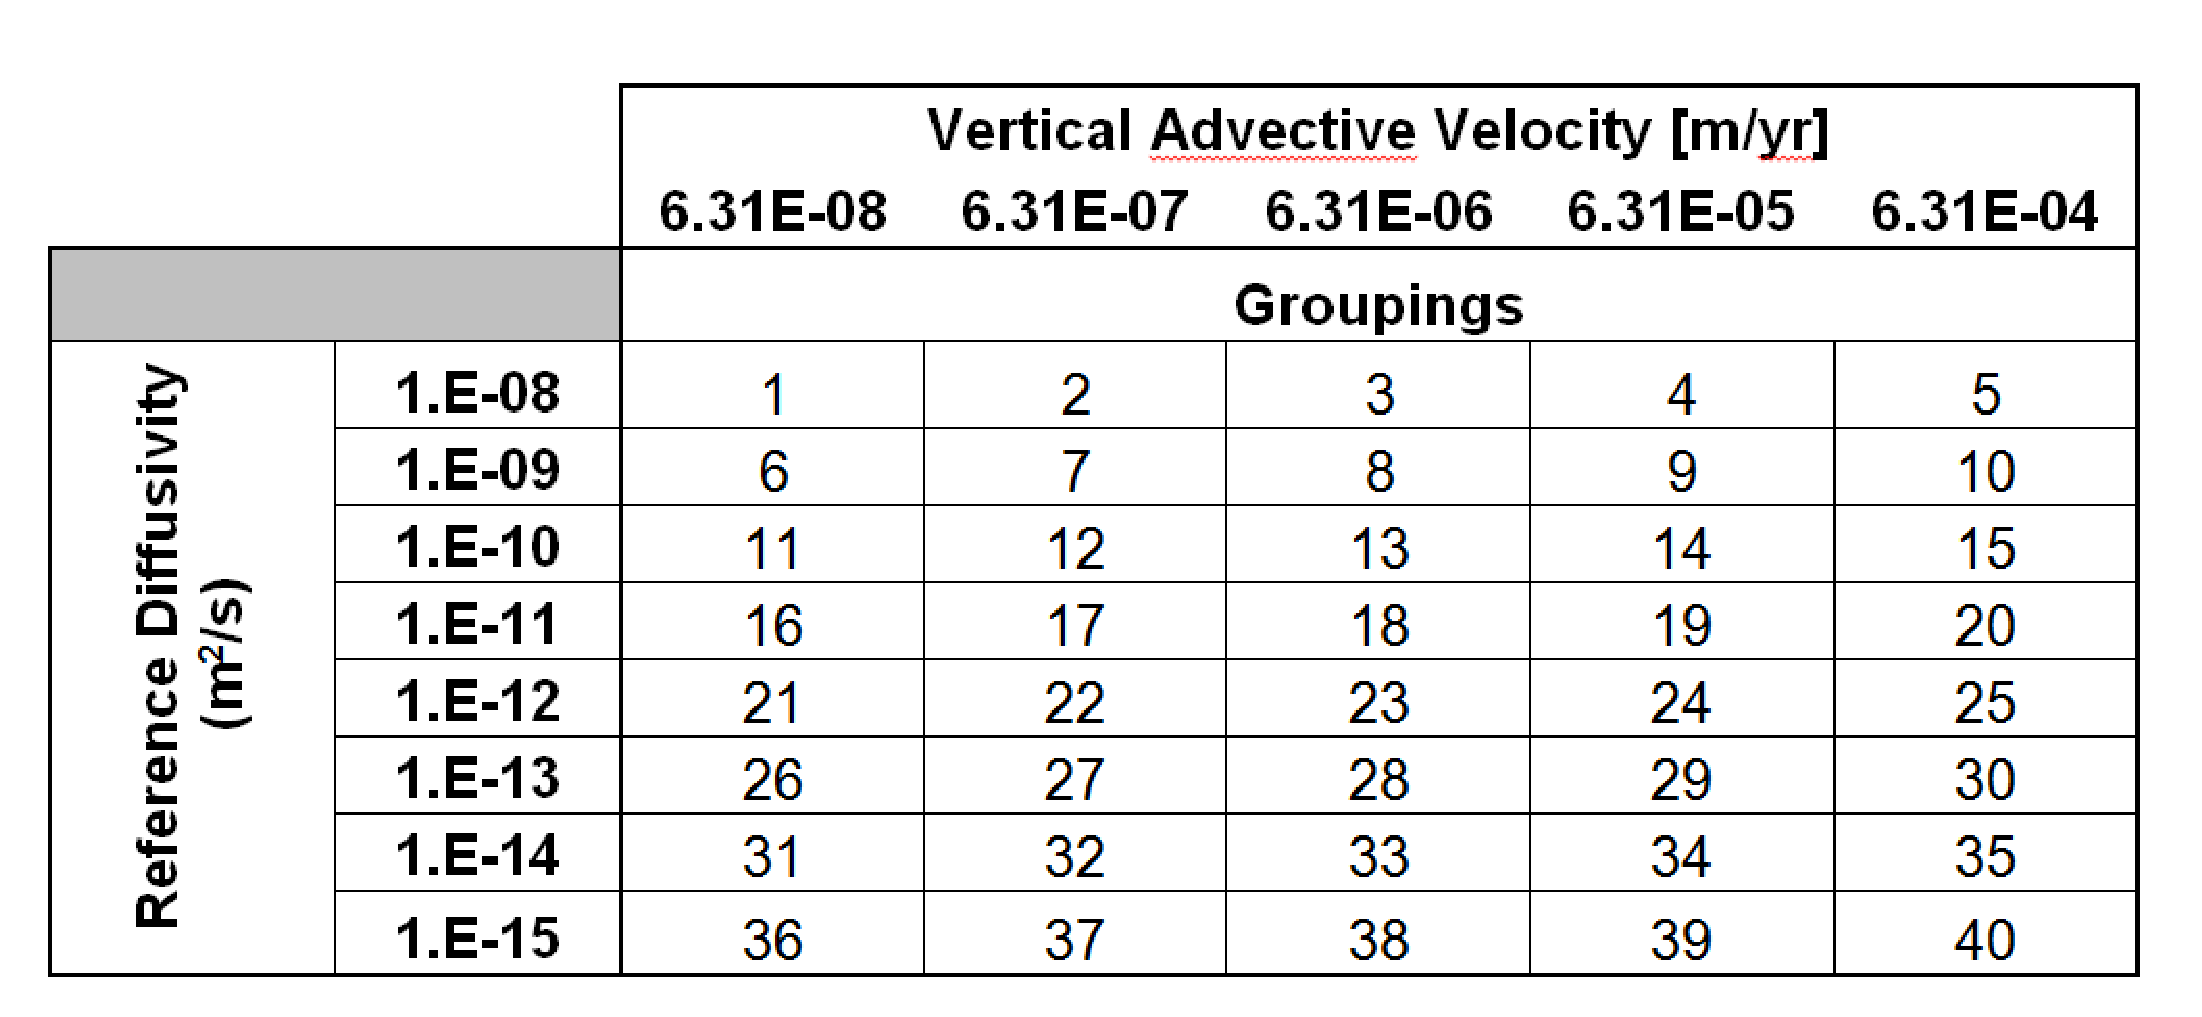
\includegraphics[width=0.8\textwidth]{AdvVelAndDiffCoeffEBSFail/AdvVelAndDiffCoeffGroups.eps}
\caption{Vertical advective velocity and diffusion coefficient simulation groupings.}
\label{tab:AdvVelAndDiffCoeffGroups}
\end{table}
\end{frame}

\begin{frame}[c]
  \frametitle{Case II : Vertical Advective Velocity and Diffusion Coefficient}
\begin{figure}[htp!]
\centering
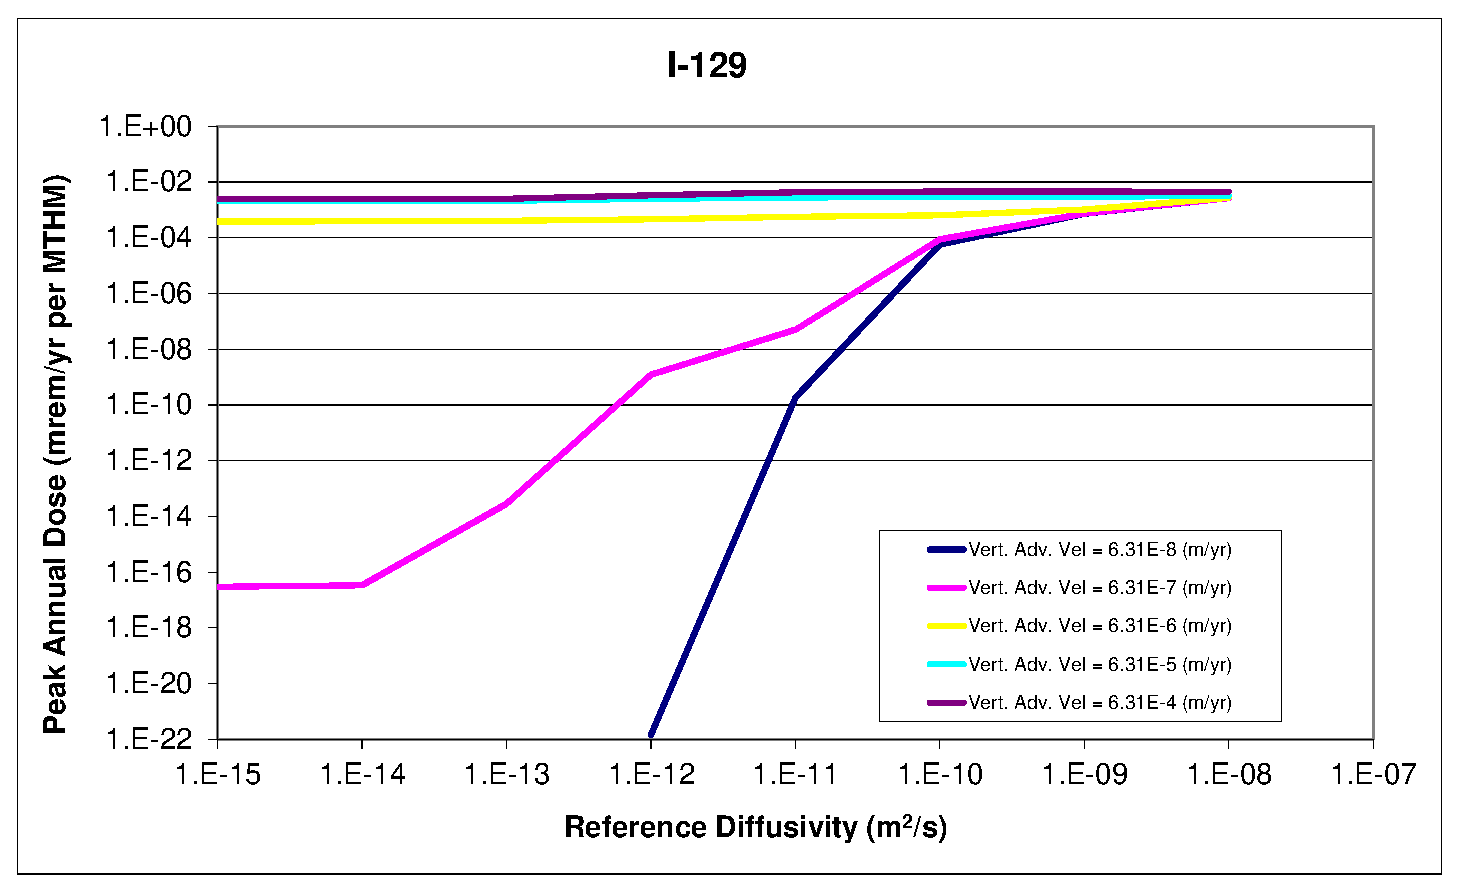
\includegraphics[width=0.8\textwidth]{AdvVelAndDiffCoeffEBSFail/I-129.eps}
\caption{$^{129}I$. For vertical advective velocities 
$6.31\times10^{-6}[m/yr]$ and above, lower reference diffusivities are 
ineffective at attenuating the mean of the peak doses for soluble, non-sorbing 
elements. 
}
\label{fig:VAdvVelI129}
\end{figure}
\end{frame}

\begin{frame}[c]
  \frametitle{Case II : Vertical Advective Velocity and Diffusion Coefficient}
\begin{figure}[htp!]
\centering
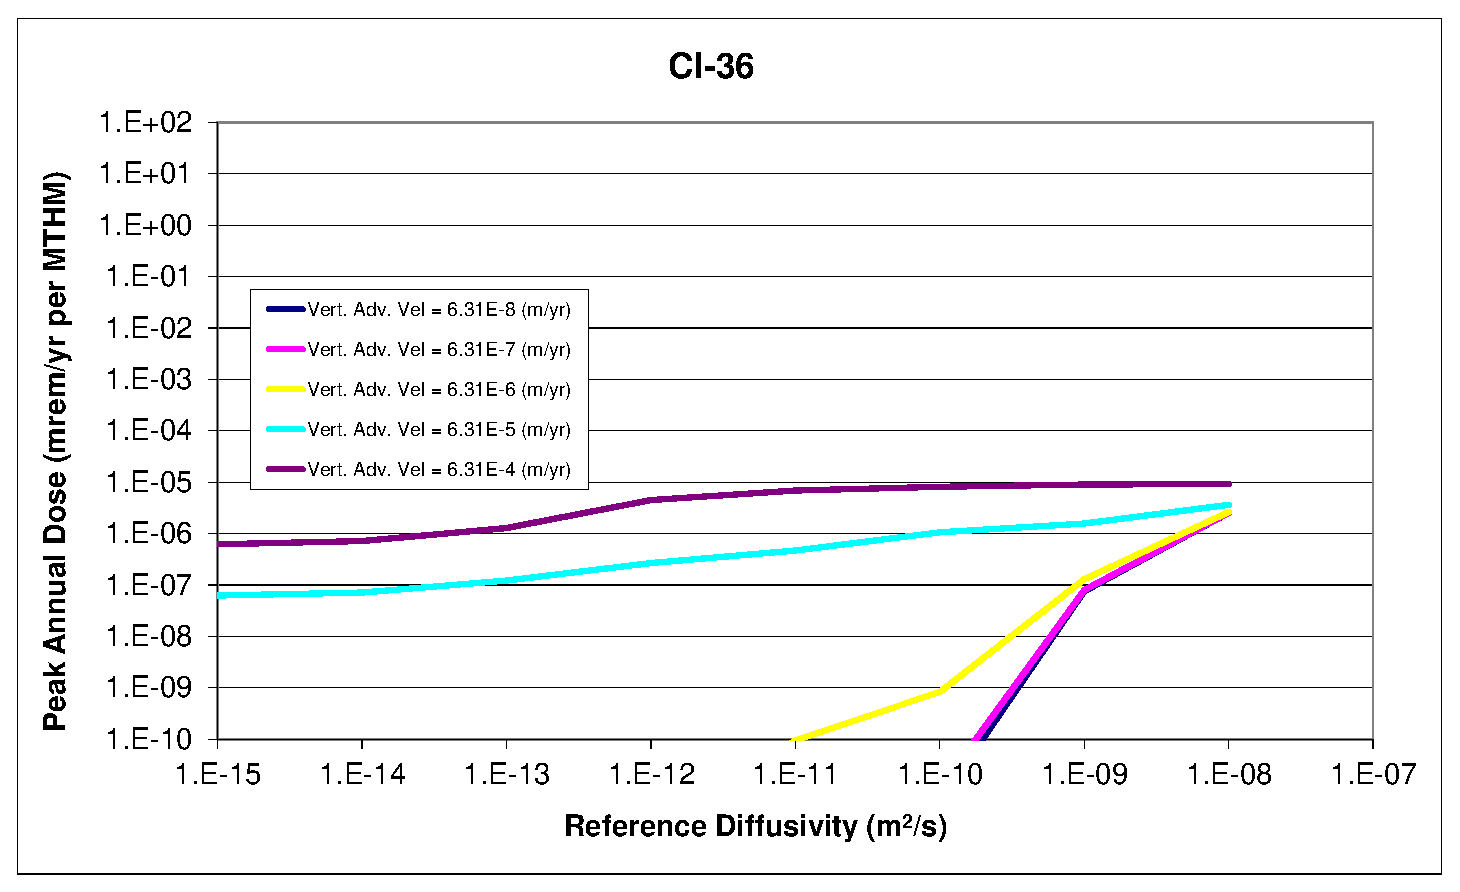
\includegraphics[width=0.8\textwidth]{AdvVelAndDiffCoeffEBSFail/Cl-36.eps}
\caption{$^{36}Cl$.
For vertical advective velocities 
$6.31\times10^{-6}[m/yr]$ and above, lower reference diffusivities are 
ineffective at attenuating the mean of the peak doses for soluble, non-sorbing 
elements. 
}
\label{fig:VAdvVelCl36}
\end{figure}
\end{frame}


\begin{frame}[c]
  \frametitle{Case II : Vertical Advective Velocity and Diffusion Coefficient}

\begin{figure}[ht!]
\centering
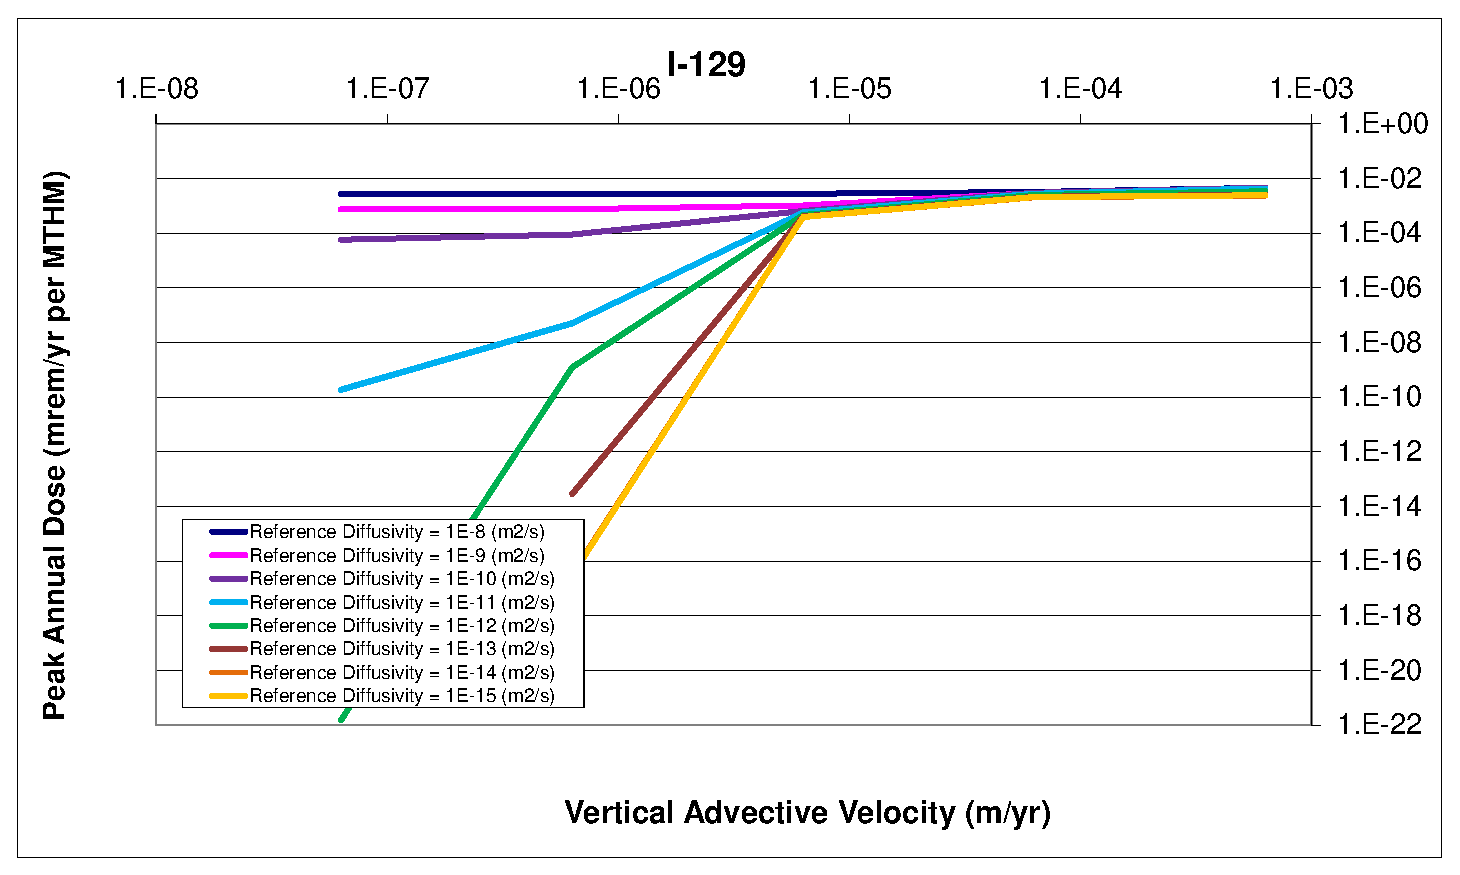
\includegraphics[width=0.8\textwidth]{AdvVelAndDiffCoeffEBSFail/I-129-VAdvVel.eps}
\caption{$^{129}I$.
For vertical advective velocities 
$6.31\times10^{-6}[m/yr]$ and above, lower reference diffusivities are 
ineffective at attenuating the mean of the peak doses for soluble, non-sorbing 
elements. 
}
\label{fig:VAdvVelI129VAdvVel}
\end{figure}
\end{frame}



\begin{frame}[c]
  \frametitle{Case II : Vertical Advective Velocity and Diffusion Coefficient}
\begin{figure}[ht!]
\centering
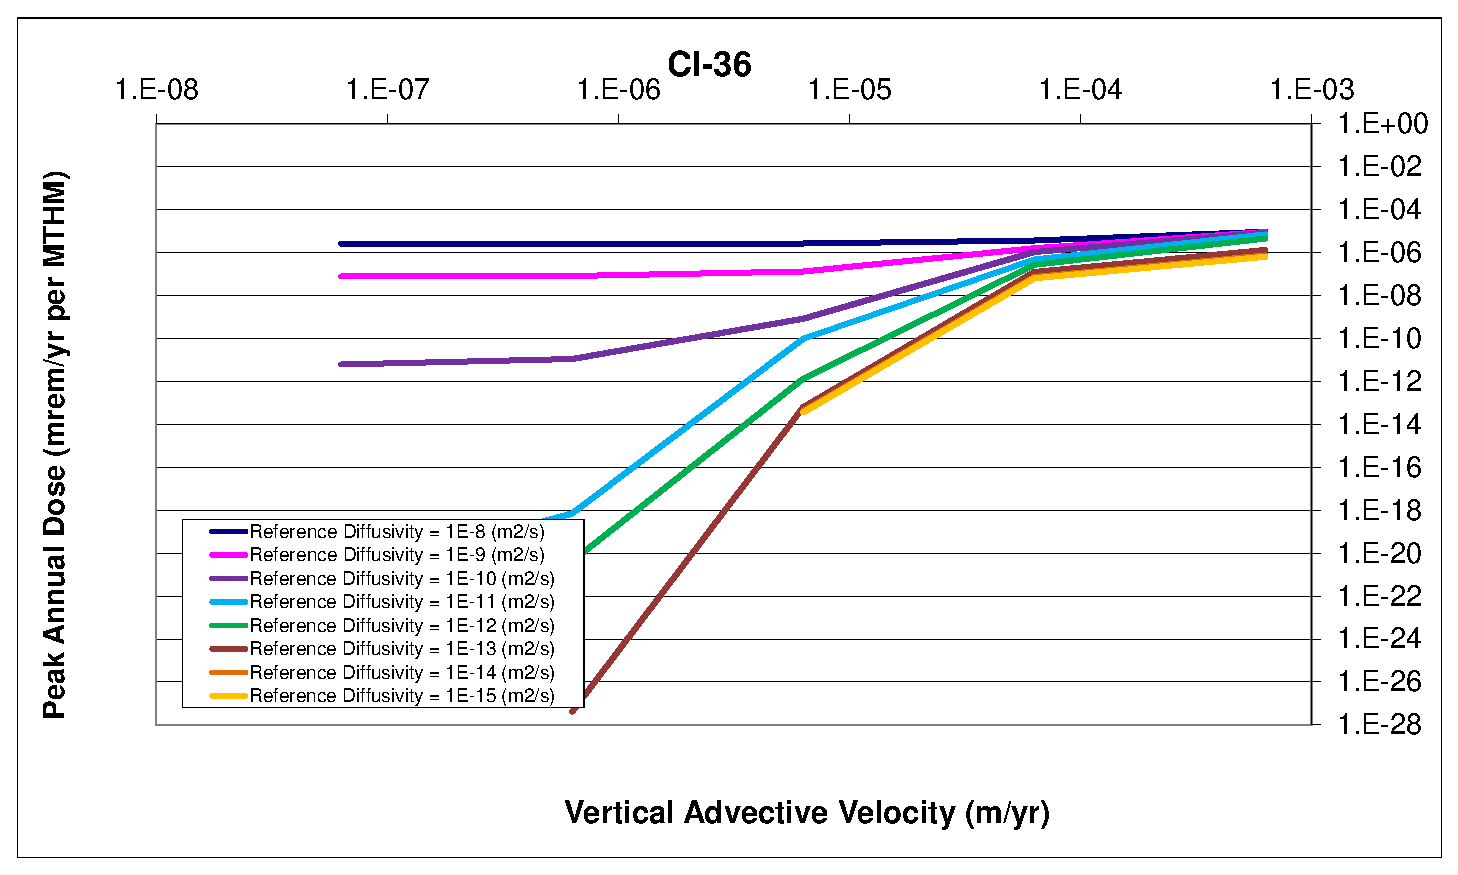
\includegraphics[width=0.8\textwidth]{AdvVelAndDiffCoeffEBSFail/Cl-36-VAdvVel.eps}
\caption{$^{36}Cl$.
For vertical advective velocities 
$6.31\times10^{-6}[m/yr]$ and above, lower reference diffusivities are 
ineffective at attenuating the mean of the peak doses for soluble, non-sorbing 
elements. 
}
\label{fig:VAdvVelCl36VAdvVel}
\end{figure}
\end{frame}

\begin{frame}[c]
  \frametitle{Case II : Vertical Advective Velocity and Diffusion Coefficient}
The solubility limited and sorbing elements, $Tc$ and $Np$, in Figures 
\ref{fig:VAdvVelTc99}, \ref{fig:VAdvVelTc99VAdvVel}, \ref{fig:VAdvVelNp237}, and 
\ref{fig:VAdvVelNp237VAdvVel}

Dose contribution from $^{99}Tc$ has a proportional 
relationship with vertical advective velocity above a regime threshold at 
$6.31\times10^{-5}[m/yr]$, above which the system exhibits sensitivity to 
advection. 

%There is an interesting feature in which $^{99}Tc$ 
%exhibits a decrease in peak annual dose for an increase in reference diffusivity 
%for the very high ($6.31\times10^{-4}$) vertcial advective velocity case. %WHY? 
\end{frame}

\begin{frame}[c]
  \frametitle{Case II : Vertical Advective Velocity and Diffusion Coefficient}
\begin{figure}[htp!]
\centering
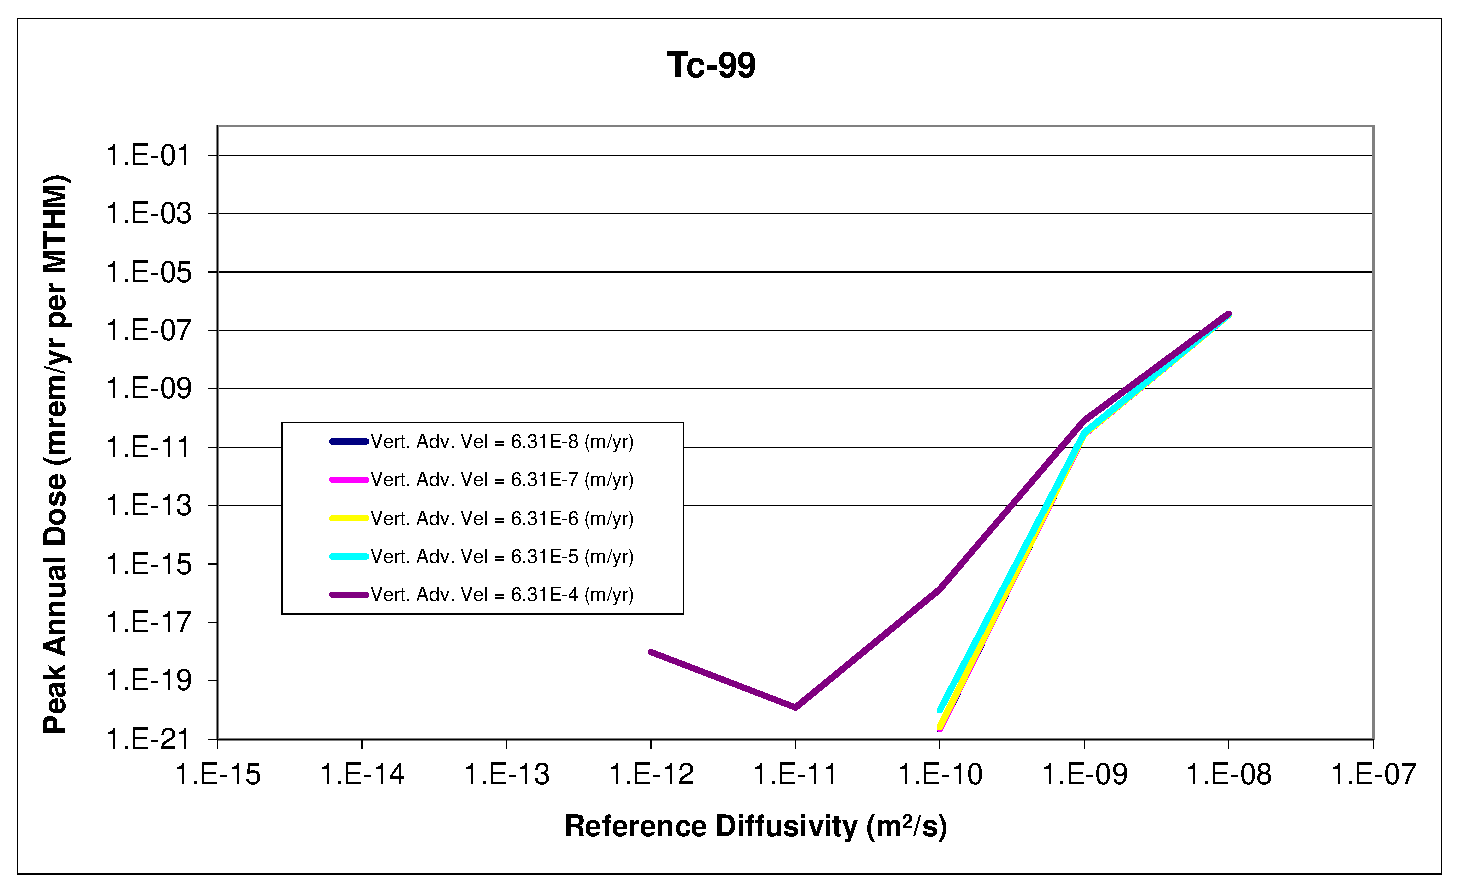
\includegraphics[width=0.8\textwidth]{AdvVelAndDiffCoeffEBSFail/Tc-99.eps}
\caption{$^{99}Tc$ 
shows a very weak influence on peak annual dose 
rate for low reference diffusivities, but a direct proportionality between 
dose and reference diffusivity above a threshold.}
\label{fig:VAdvVelTc99}
\end{figure}
\end{frame}

\begin{frame}[c]
  \frametitle{Case II : Vertical Advective Velocity and Diffusion Coefficient}
\begin{figure}[htp!]
\centering
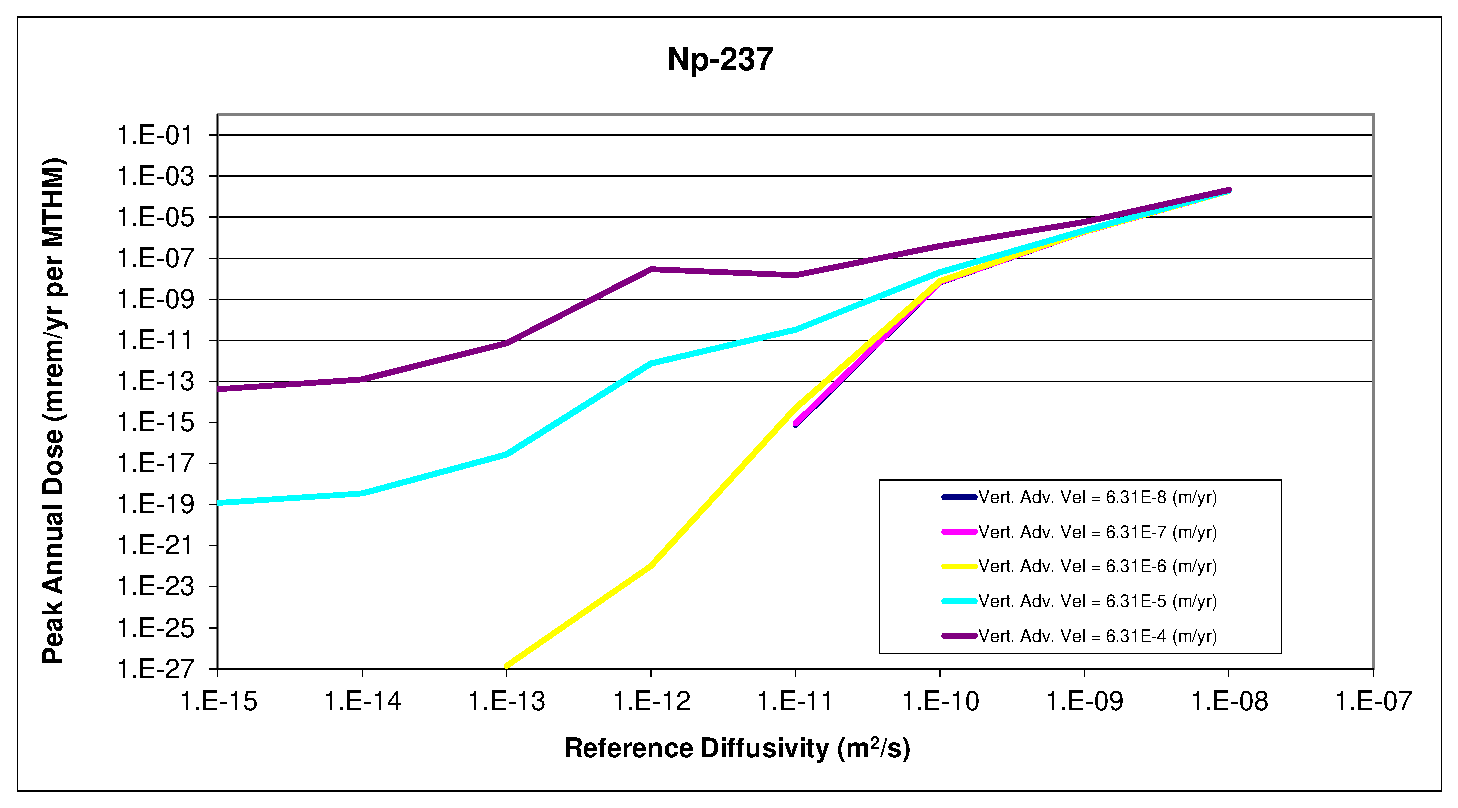
\includegraphics[width=0.8\textwidth]{AdvVelAndDiffCoeffEBSFail/Np-237.eps}
\caption{$^{237}Np$.
shows a very weak influence on peak annual dose 
rate for low reference diffusivities, but a direct proportionality between 
dose and reference diffusivity above a threshold.}
\label{fig:VAdvVelNp237}
\end{figure}
\end{frame}

\begin{frame}[c]
  \frametitle{Case II : Vertical Advective Velocity and Diffusion Coefficient}
\begin{figure}[htp!]
\centering
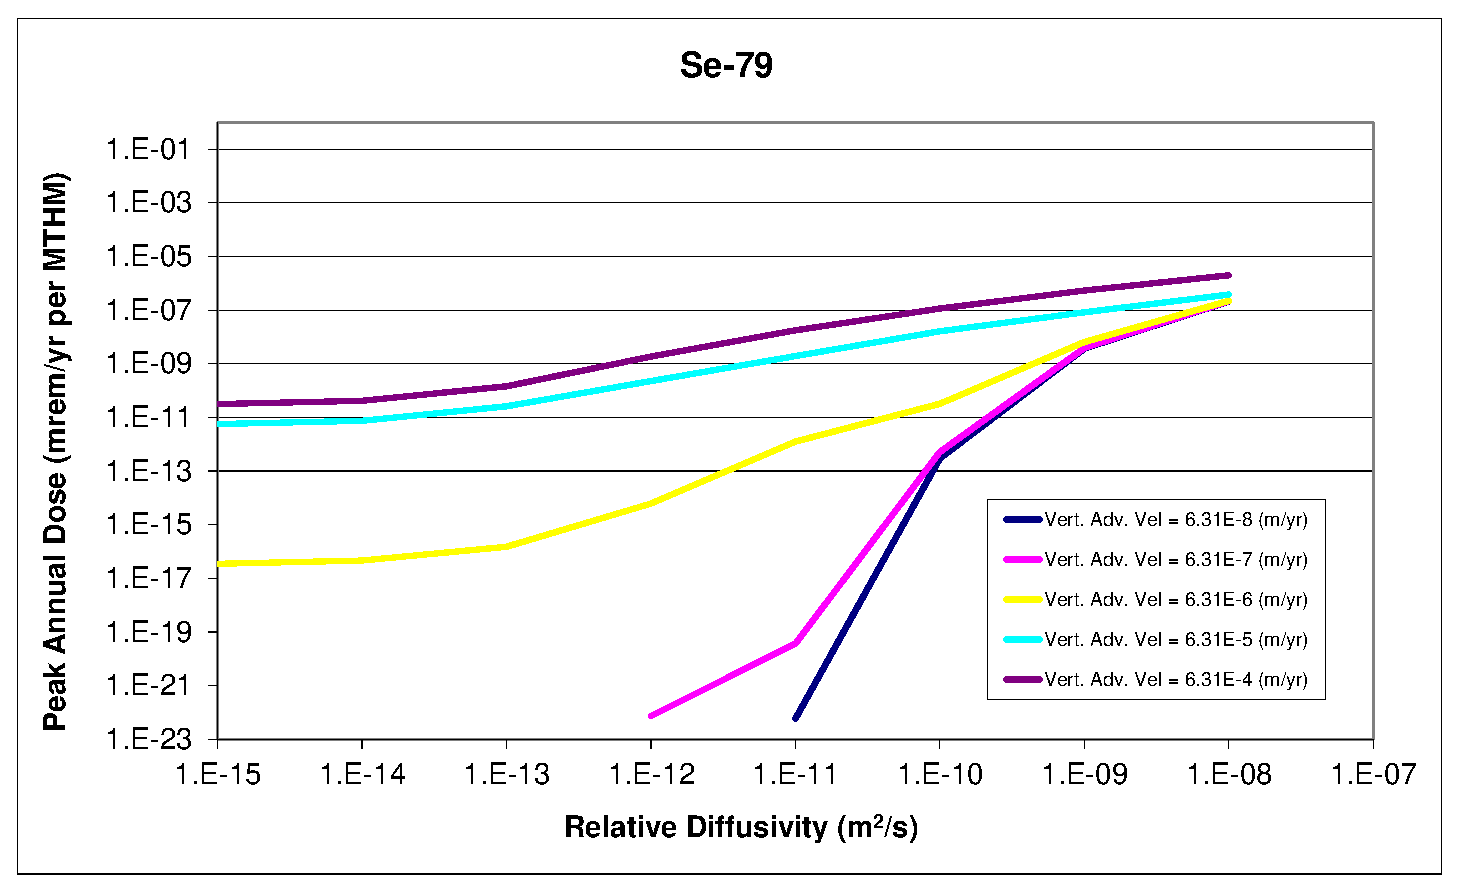
\includegraphics[width=0.8\textwidth]{AdvVelAndDiffCoeffEBSFail/Se-79.eps}
\caption{$^{79}Se$.
$Se$ is non sorbing, but solubility limited.  
For low vertical advective velocity, 
the system is diffusion dominated.}
\label{fig:VAdvVelSe79}
\end{figure}
\end{frame}


\begin{frame}[c]
  \frametitle{Case II : Vertical Advective Velocity and Diffusion Coefficient}
\begin{figure}[ht!]
\centering
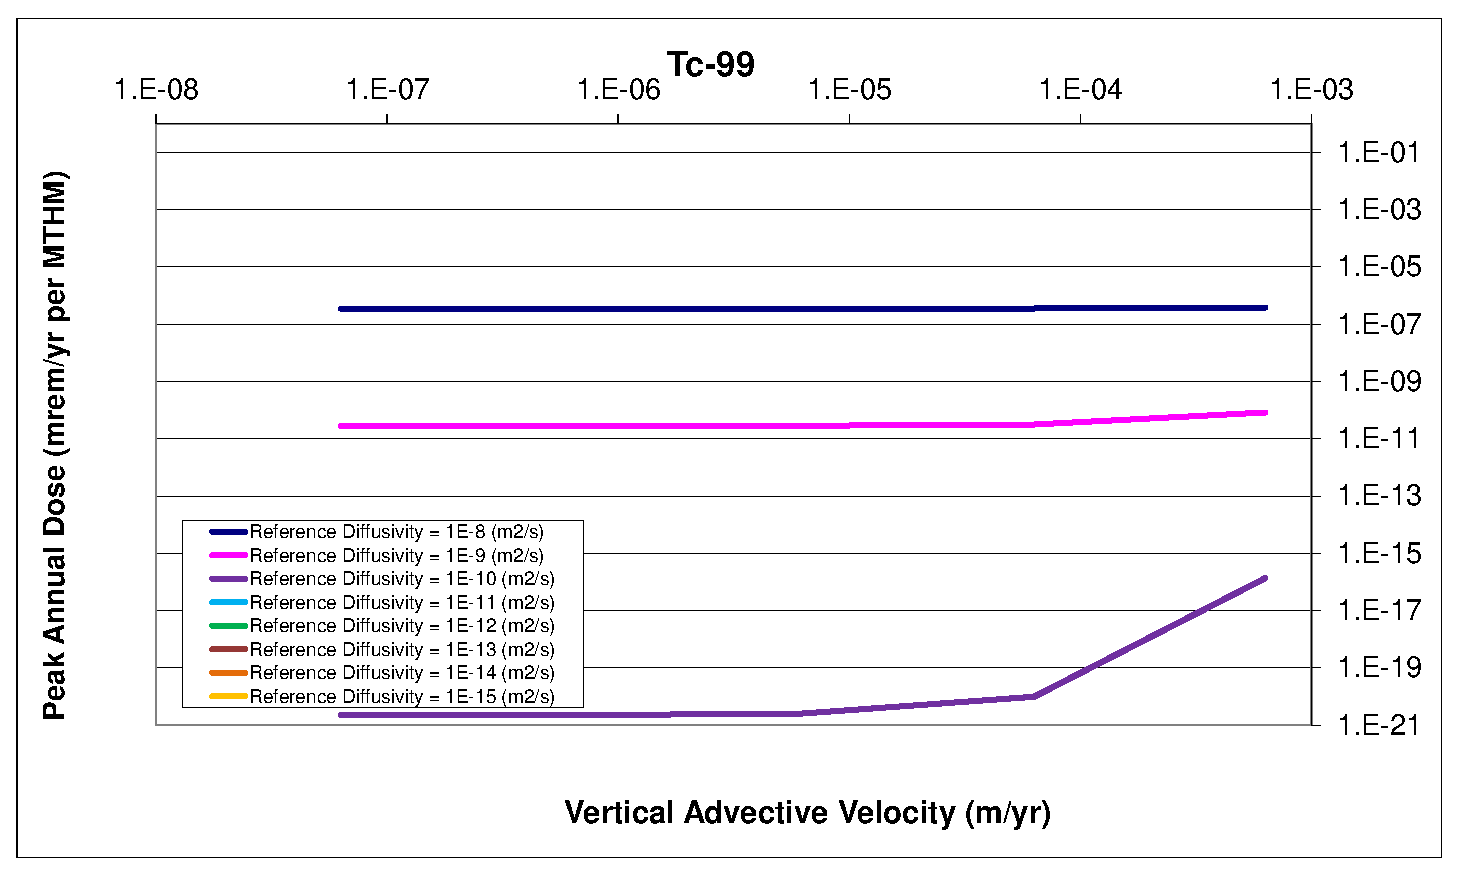
\includegraphics[width=0.8\textwidth]{AdvVelAndDiffCoeffEBSFail/Tc-99-VAdvVel.eps}
\caption{$^{99}Tc$.
shows a very weak influence on peak annual dose 
rate for low reference diffusivities, but a direct proportionality between 
dose and reference diffusivity above a threshold.}
\label{fig:VAdvVelTc99VAdvVel}
\end{figure}
\end{frame}


\begin{frame}[c]
  \frametitle{Case II : Vertical Advective Velocity and Diffusion Coefficient}
\begin{figure}[ht!]
\centering
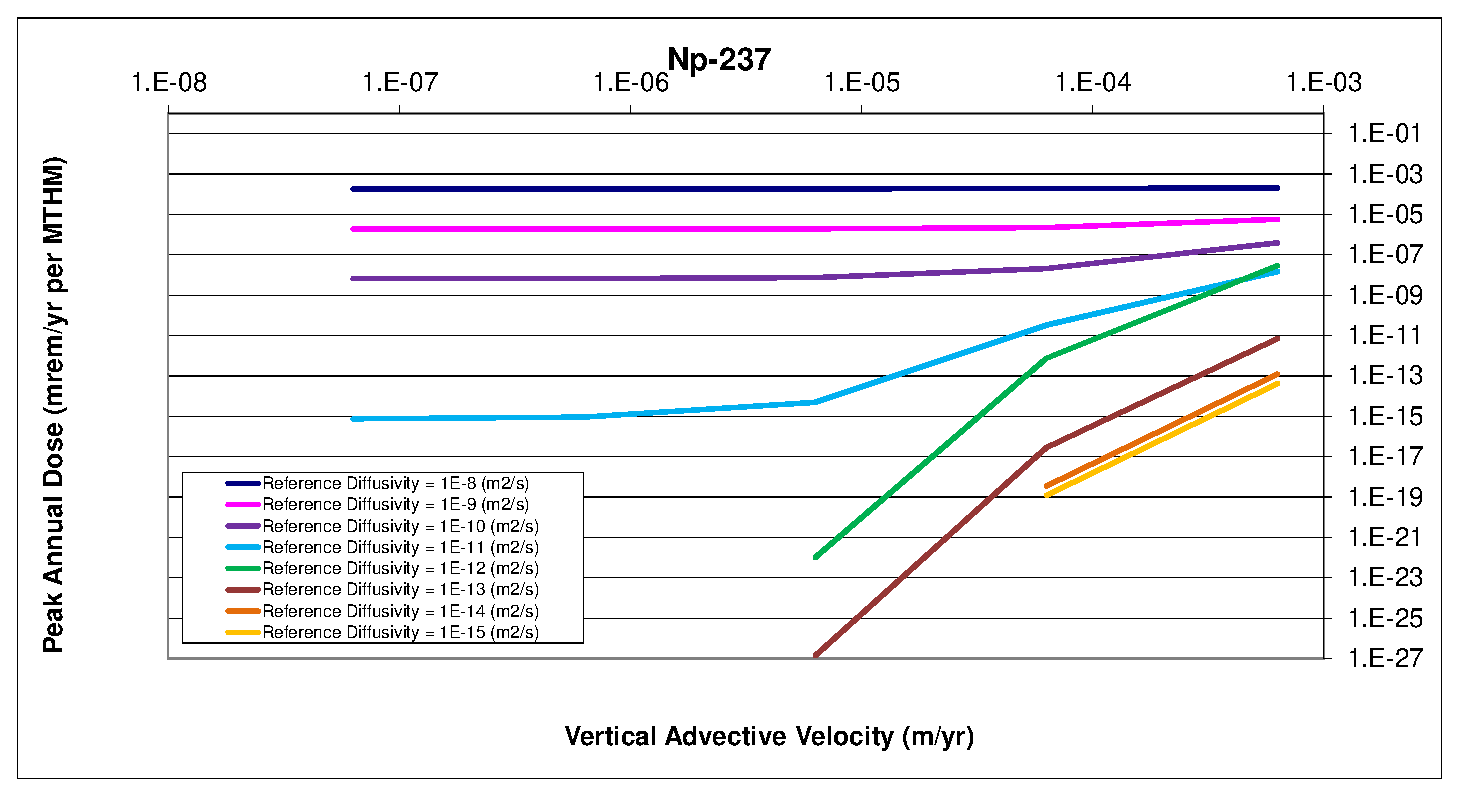
\includegraphics[width=0.8\textwidth]{AdvVelAndDiffCoeffEBSFail/Np-237-VAdvVel.eps}
\caption{$^{237}Np$.
shows a very weak influence on peak annual dose 
rate for low reference diffusivities, but a direct proportionality between 
dose and reference diffusivity above a threshold.}
\label{fig:VAdvVelNp237VAdvVel}
\end{figure}
\end{frame}

\begin{frame}[c]
  \frametitle{Case II : Vertical Advective Velocity and Diffusion Coefficient}
\begin{figure}[ht!]
\centering
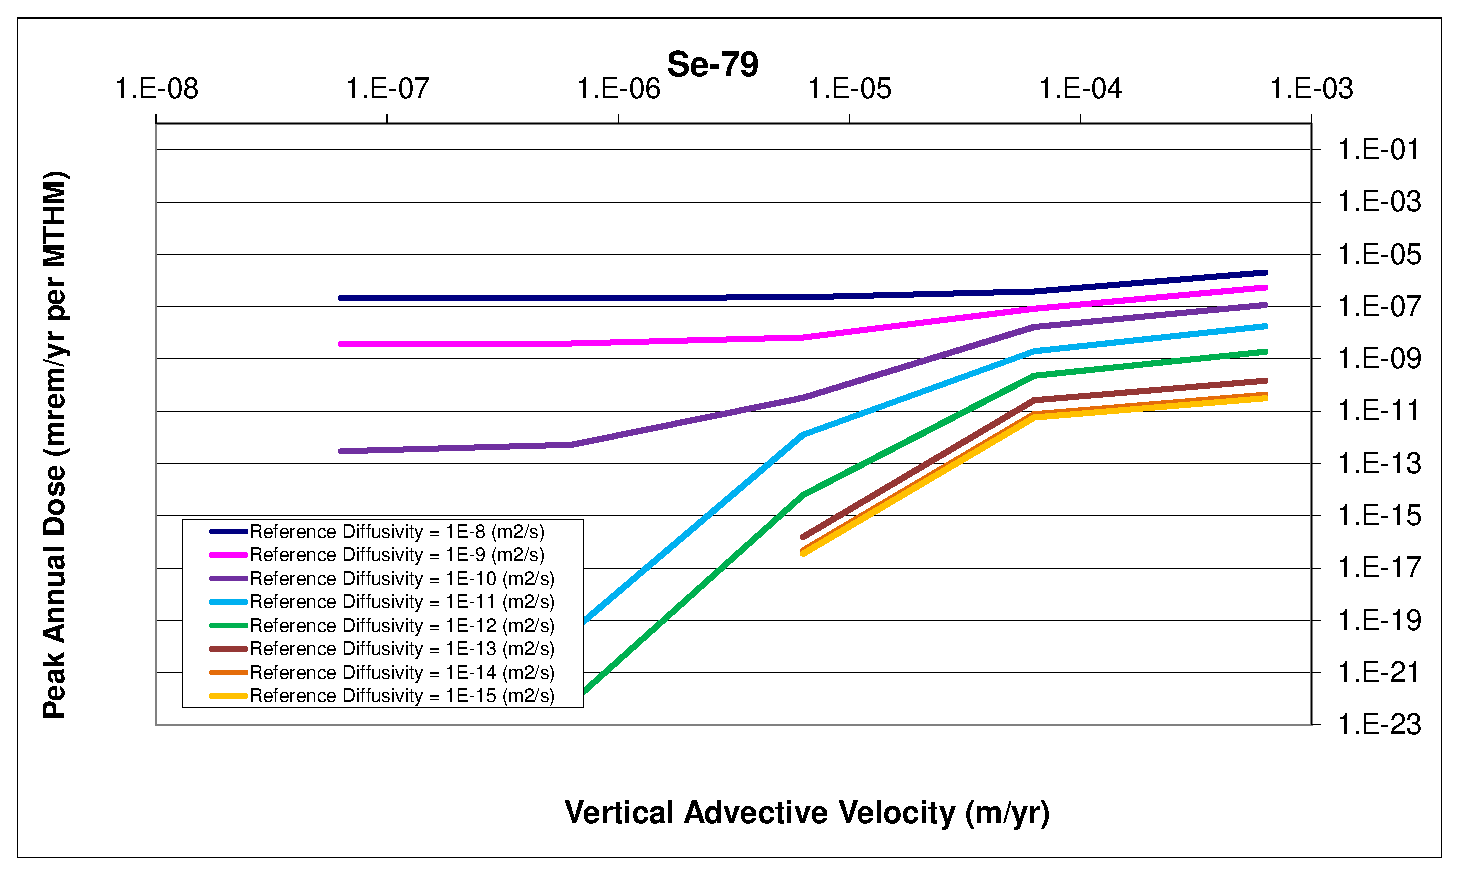
\includegraphics[width=0.8\textwidth]{AdvVelAndDiffCoeffEBSFail/Se-79-VAdvVel.eps}
\caption{$^{79}Se$.
$Se$ is non sorbing, but solubility limited.  
For high vertical advective 
velocity, the diffusivity remains important even in the advective regime as 
spreading facilitates transport in the presence of solubility limited transport. 
vertical advective velocity sensitivity.}
\label{fig:VAdvVelSe79VAdvVel}
\end{figure}
\end{frame}



\subsection{Case III : Solubility Coefficients}

The dissolution behavior of a solute in an aqueous solution is called its 
solubility. This behavior is restricted by the solute's solubility limit, described  
by an equilibrium constant that depends upon temperature, water chemistry, and 
the properties of the element. 

For modeling simplicity, the solubility limit of each isotope, $i$, was assumed 
to have a solubility limit, $S_i$, equal to the elemental solubility limit of 
the associated element.  By varying the multiplication factor applied to the 
expected solubility limit, $\langle S_i\rangle$, this analysis varied solubility 
limit for each isotope $i$, as detailed in Table \ref{tab:Cases}.  This method 
preserves, in some sense, the relative solubility limits between isotopes, which 
vary over many magnitudes.  

As seen in Figure \ref{fig:SolSum}, for solubility limits below a threshold, 
approximately $1\times10^{-10}[mol\cdot m^{-3}]$, dose releases were directly 
and strongly proportional to the solubility limit. This indicated that the 
radionuclide concentration saturated the groundwater up to the solubility limit 
near the waste form.  For solubility limits above the threshold, however, 
further increase to the limit had no effect on the peak dose. This demonstrated 
the situation in which the solubility limit was so high that even complete 
dissolution of the waste inventory into the pore water was insufficient to reach 
the solubility limit.

\begin{figure}[H]
  \centering
  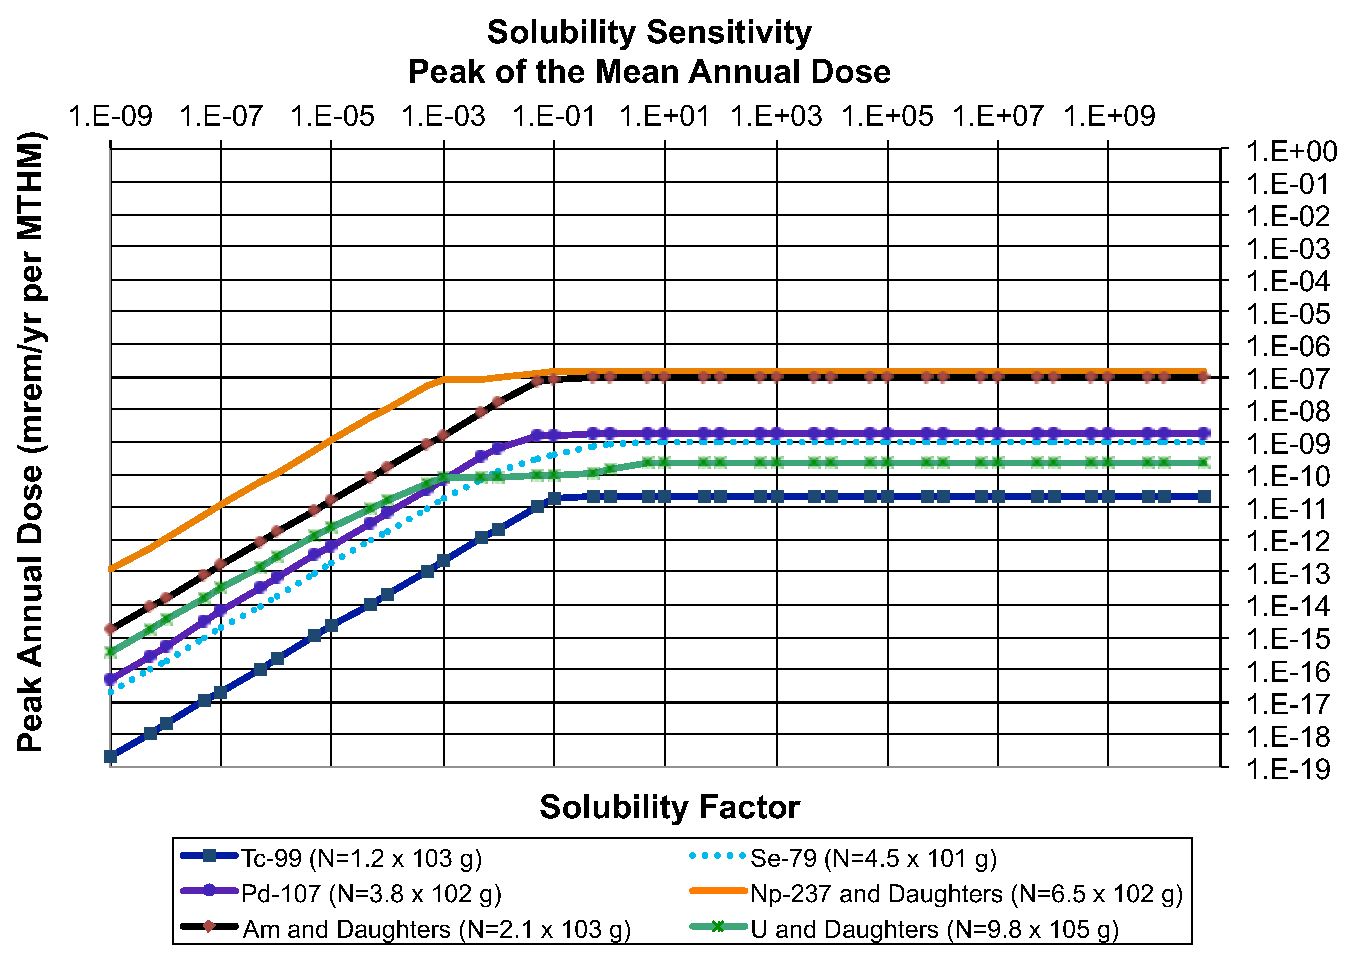
\includegraphics[width=\linewidth]{solubility.eps}
  \caption{Solubility limit sensitivity. The peak annual dose due to an 
  inventory, 
  $N$, of each isotope.}
  \label{fig:SolSum}
\end{figure}



\subsection{Case IV : Partition Coefficient}

This analysis investigated the sensitivity of repository performance to
to the elemental partition coefficient. 

The partition or distribution coefficient, $K_d$, relates the amount of contaminant adsorbed into the 
solid phase of the host medium to the amount of contaminant adsorbed into the 
aqueous phase of the host medium. It is a common empirical coefficient used to 
capture the effects of a number of retardation mechanisms. The coefficient 
$K_{d,i}$, in units of $[m^3\cdot kg^{-1}]$, is the ratio of the mass of 
contaminant $i$ in the solid to the mass of contaminant $i$ in the solution.

As indicated in Table \ref{tab:Cases}, the parameters in this model were all set 
to the default values except a multiplier applied to the expect partitioning 
coefficients, $\langle K_{d,i} \rangle$, for each isotope $i$. This multiplier 
preserved, in some sense, the widely varying 
relative sorption behavior among elements. 

The expected inverse relationship between the partition coefficient resulting 
peak annual dose was found for all elements that were not assumed to be 
effectively infinitely soluble.  It is clear from Figure \ref{fig:KdSum} that 
for partition coefficients greater than a threshold, approximately 
  $1\pm10[m^3\cdot kg^{-1}]$ the relationship between 
peak annual dose and partition coefficient is a strong inverse one. 

\begin{figure}[ht]
  \centering
  \includegraphics[width=\linewidth]{Partitioning_Summary.eps}
  \caption{$K_d$ sensitivity.  The peak annual dose due to an inventory, 
  $N$, of each isotope.}
  \label{fig:KdSum}
\end{figure}



\begin{frame}[c]
  \frametitle{Case V : Waste Form Degradation Rate and Inventory}
These runs varied the waste form degradation rate and the waste inventory mass 
factor.  There were forty runs corresponding to eight values of the waste form degradation 
rate and five values of the mass factor.

\begin{table}[ht!]
\centering
\footnotesize{
\begin{tabular}{|l|l|l|r|r|}
\multicolumn{5}{c}{\textbf{Simulation Cases}}\\
\hline
\textbf{Case} & \textbf{Parameter} & \textbf{Units} & \textbf{Min. Value} & \textbf{Max. Value}\\
\hline
V     & $R_{WFDeg.}$           & $[yr^{-1}]$       & $10^{-9}$    &  $10^{-2}$ \\
      & Inventory              & [MTHM]         & $10^{-4}$    &  $10^1$ \\
\hline
\end{tabular}
\caption{Each dual and single parameter simulation case had 40 simulation 
groups of 100 realizations each.}
\label{tab:Cases}
}
\end{table}


\end{frame}

\begin{frame}[c]
  \frametitle{Case V : Waste Form Degradation Rate and Inventory}

Safety indicators for post closure repository performance have been developed by 
the \gls{UFD} campaign which utilize the inventory multiplier that was varied in 
this study \cite{nutt_generic_2009}. These indicators are normalized by a 
normalization factor (100 mrem/yr) recommended by the \gls{IAEA} as the limit to 
``relevant critical members of the public'' \cite{iaea_international_1996}. The functional form for 
this safety indicator for a single waste category, \gls{HLW}, is just 

\begin{align}
SI_{G} &= \left(\frac{\sum_{i=1}^{N}D_{G,i}(I_i, F_{d})}{100mrem/yr}\right)[GWe/yr].
\label{indicator}
\intertext{where}
SI_{G} &= \mbox{Safety indicator for disposal in media type G}[GWe/yr]\nonumber\\
N &= \mbox{Number of key radionuclides considered in this indicator}\nonumber\\
D_{G,i} &= \mbox{Peak dose rate from isotope i in media type G}[mrem/yr]\nonumber\\
F_{d} &= \mbox{Fractional waste form degradation rate}[1/yr].\nonumber
\end{align}
\end{frame}

\begin{frame}[c]
  \frametitle{Case V : Waste Form Degradation Rate and Inventory}
\begin{figure}[ht!]
\centering
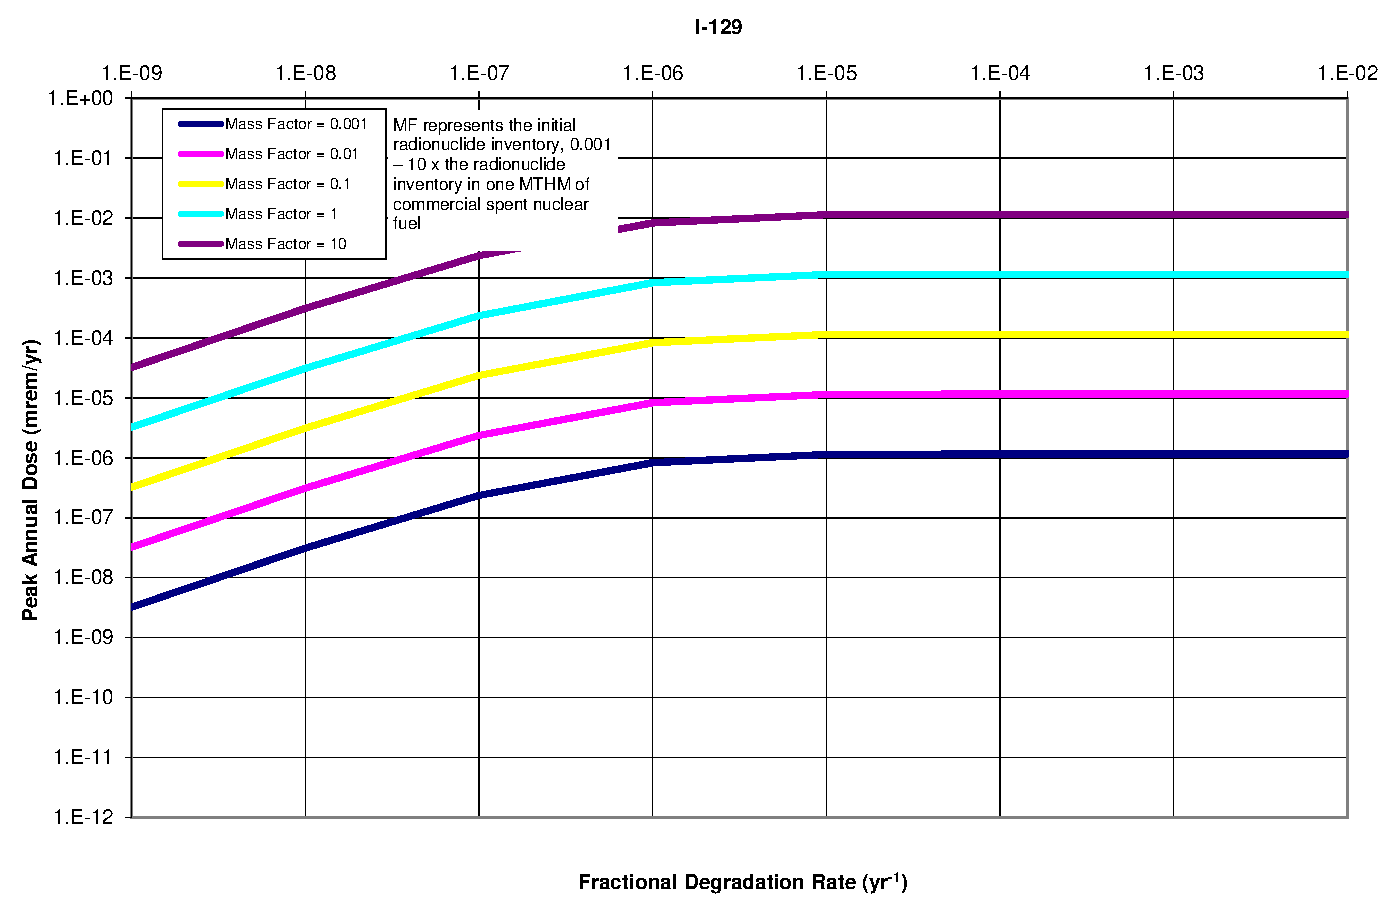
\includegraphics[width=0.8\textwidth]{WFDegAndInv/I-129.eps}
\caption{
Highly soluble and non-sorbing $^{129}I$ demonstrates a direct proportionality between dose rate and 
fractional degradation rate until a turnover where other natural system 
parameters dampen transport.} 
\label{fig:WFDegI129}
\end{figure}
\end{frame}

\begin{frame}[c]
  \frametitle{Case V : Waste Form Degradation Rate and Inventory}

\begin{figure}[ht!]
\centering
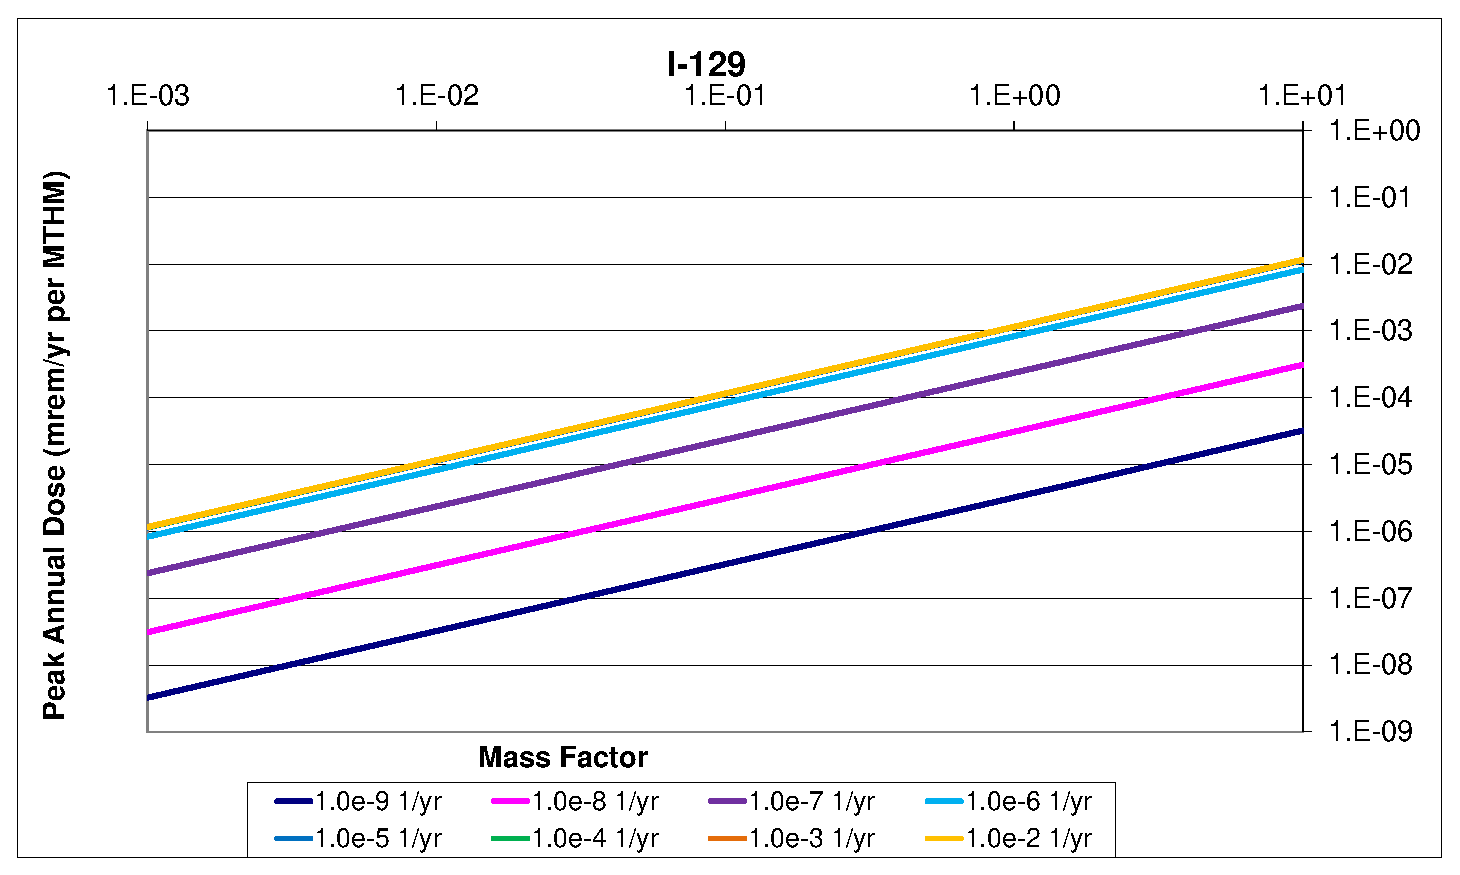
\includegraphics[width=0.8\textwidth]{WFDegAndInv/I-129-MF.eps}
\caption{
Highly soluble and non-sorbing $^{129}I$ domonstrates a direct 
proportionality to the inventory multiplier.}
\label{fig:WFDegI129MF}
\end{figure}
\end{frame}

\begin{frame}[c]
  \frametitle{Case V : Waste Form Degradation Rate and Inventory}
\begin{figure}[ht!]
\centering
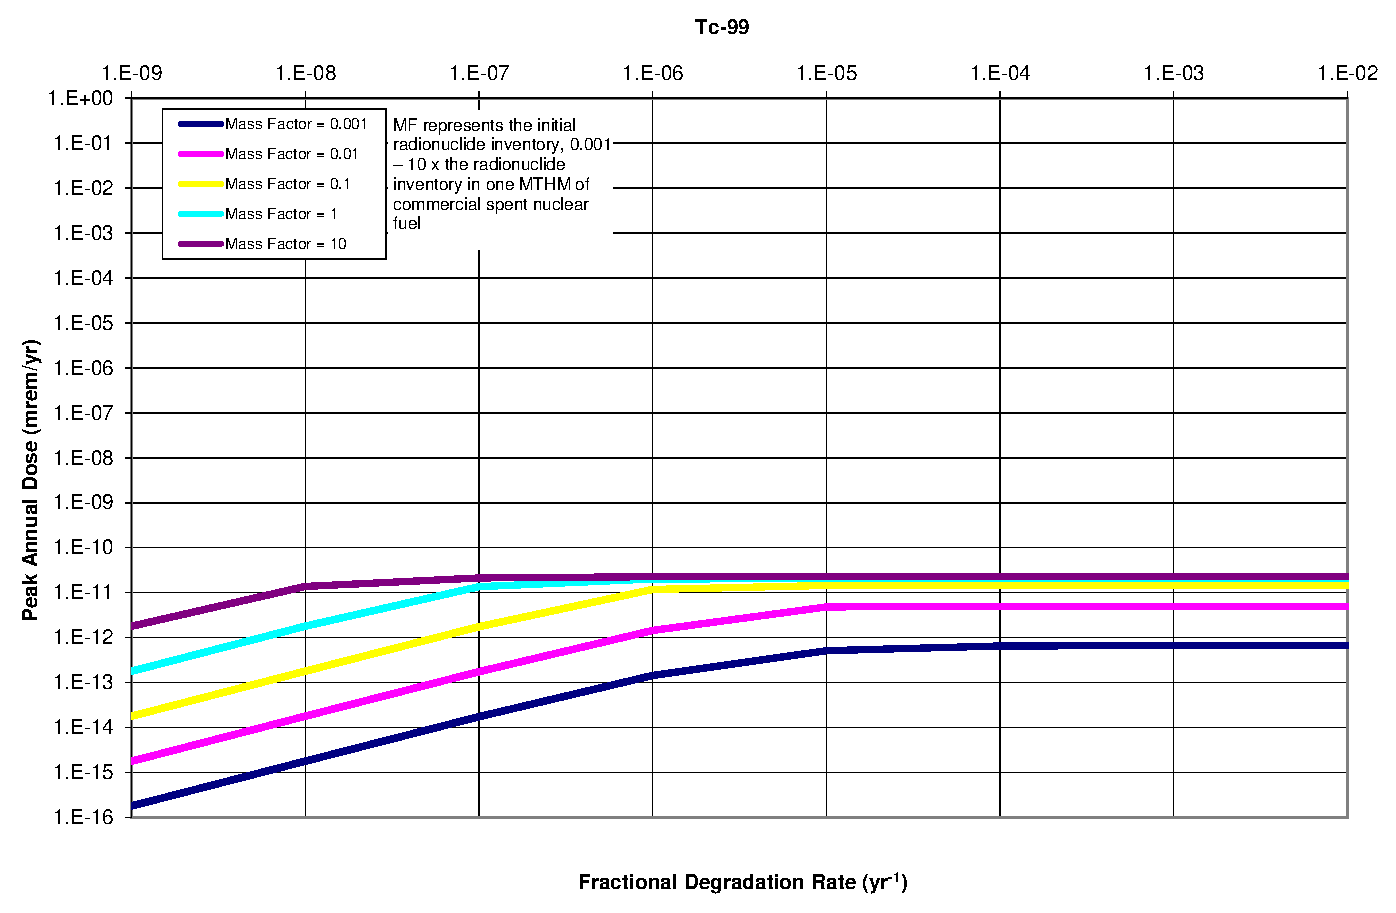
\includegraphics[width=0.8\textwidth]{WFDegAndInv/Tc-99.eps}
\caption{
Solubility limited and sorbing $^{99}Tc$ demonstrates a stronger turnover and direct proportionality 
to fractional degradation rate until attuation by its solubility limit and other 
natural system parameters. } 
\label{fig:WFDegTc99}
\end{figure}
\end{frame}

\begin{frame}[c]
  \frametitle{Case V : Waste Form Degradation Rate and Inventory}

\begin{figure}[ht!]
\centering
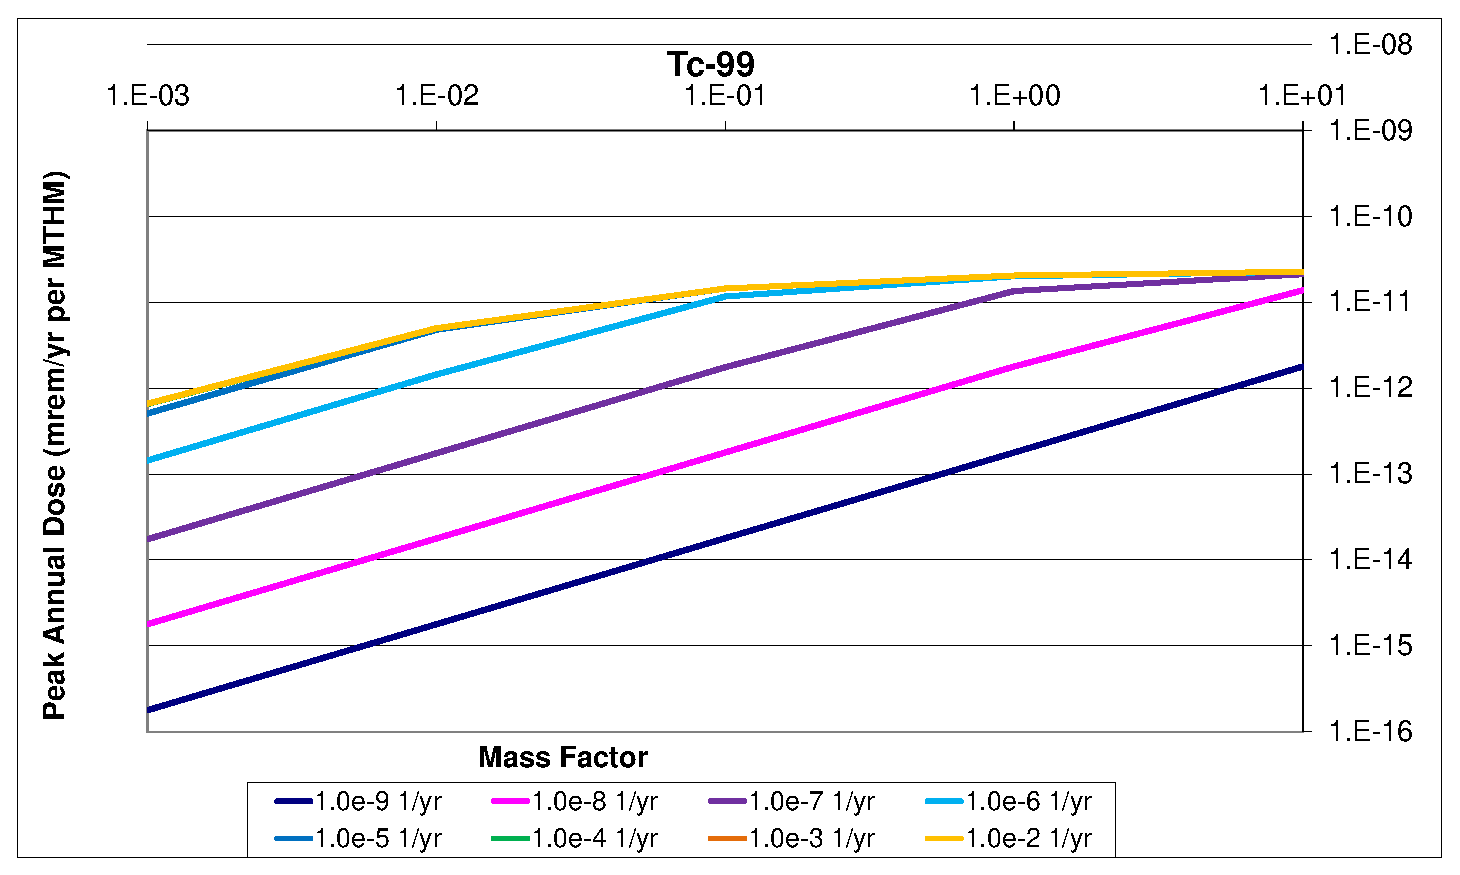
\includegraphics[width=0.8\textwidth]{WFDegAndInv/Tc-99-MF.eps}
\caption{
  Solubility limited and sorbing $^{99}Tc$ demonstrates a direct proportionality 
to fractional degradation rate until attuation by its solubility limit and other 
natural system parameters. } 
\label{fig:WFDegTc99MF}
\end{figure}

\end{frame}

\begin{frame}[c]
  \frametitle{Case V : Waste Form Degradation Rate and Inventory}

\begin{figure}[ht!]
\centering
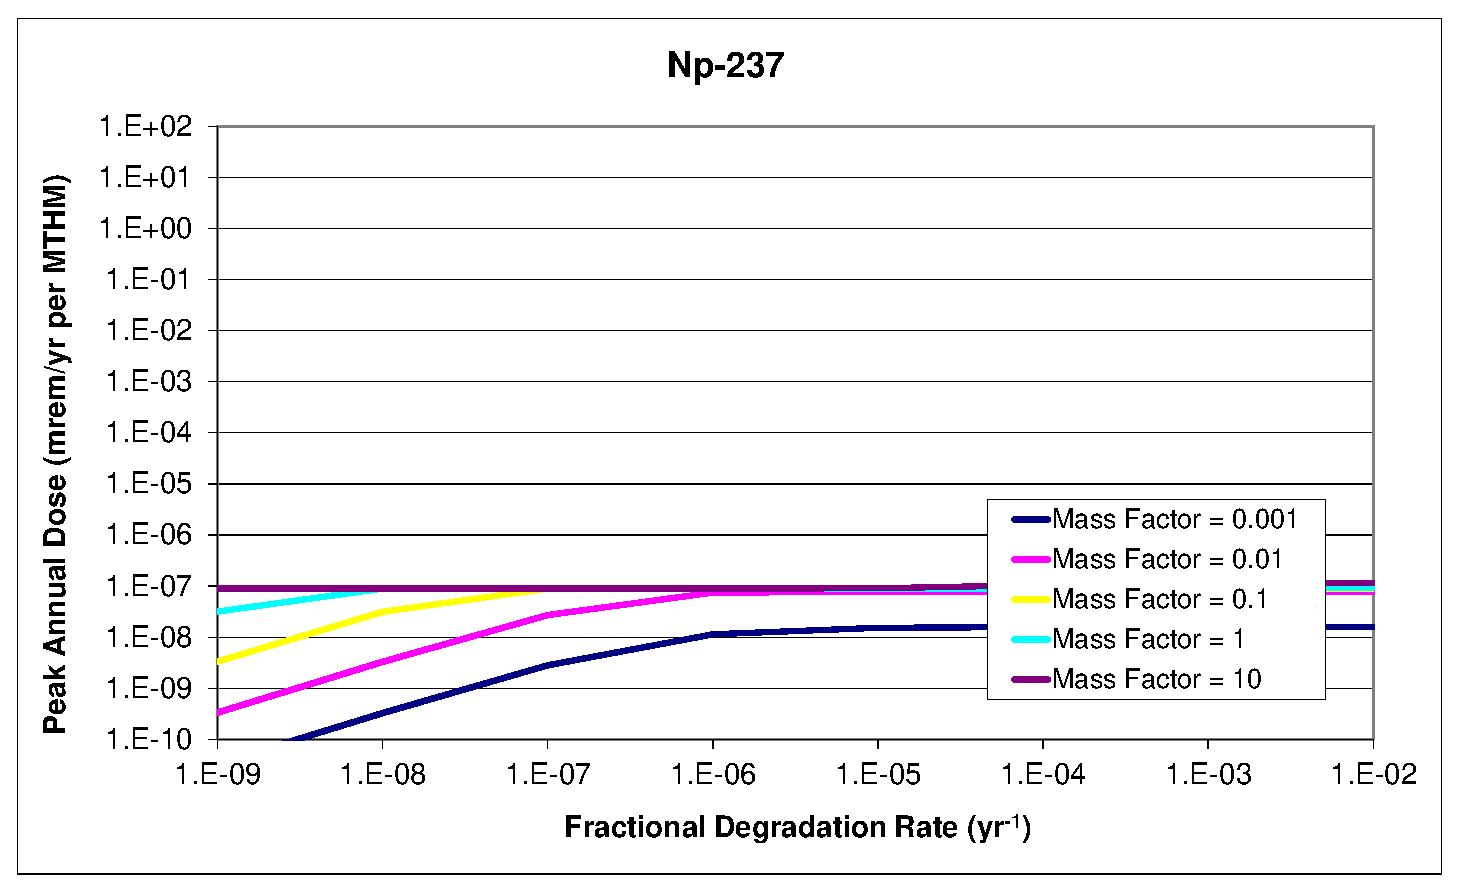
\includegraphics[width=0.8\textwidth]{WFDegAndInv/Np-237.eps}
\caption{
  Solubility limited and sorbing $^{237}Np$ demonstrates a direct proportionality 
to fractional degradation rate until attuation by its solubility limit and other 
natural system parameters. } 
\label{fig:WFDegNp237}
\end{figure}
\end{frame}

\begin{frame}[c]
  \frametitle{Case V : Waste Form Degradation Rate and Inventory}

\begin{figure}[ht!]
\centering
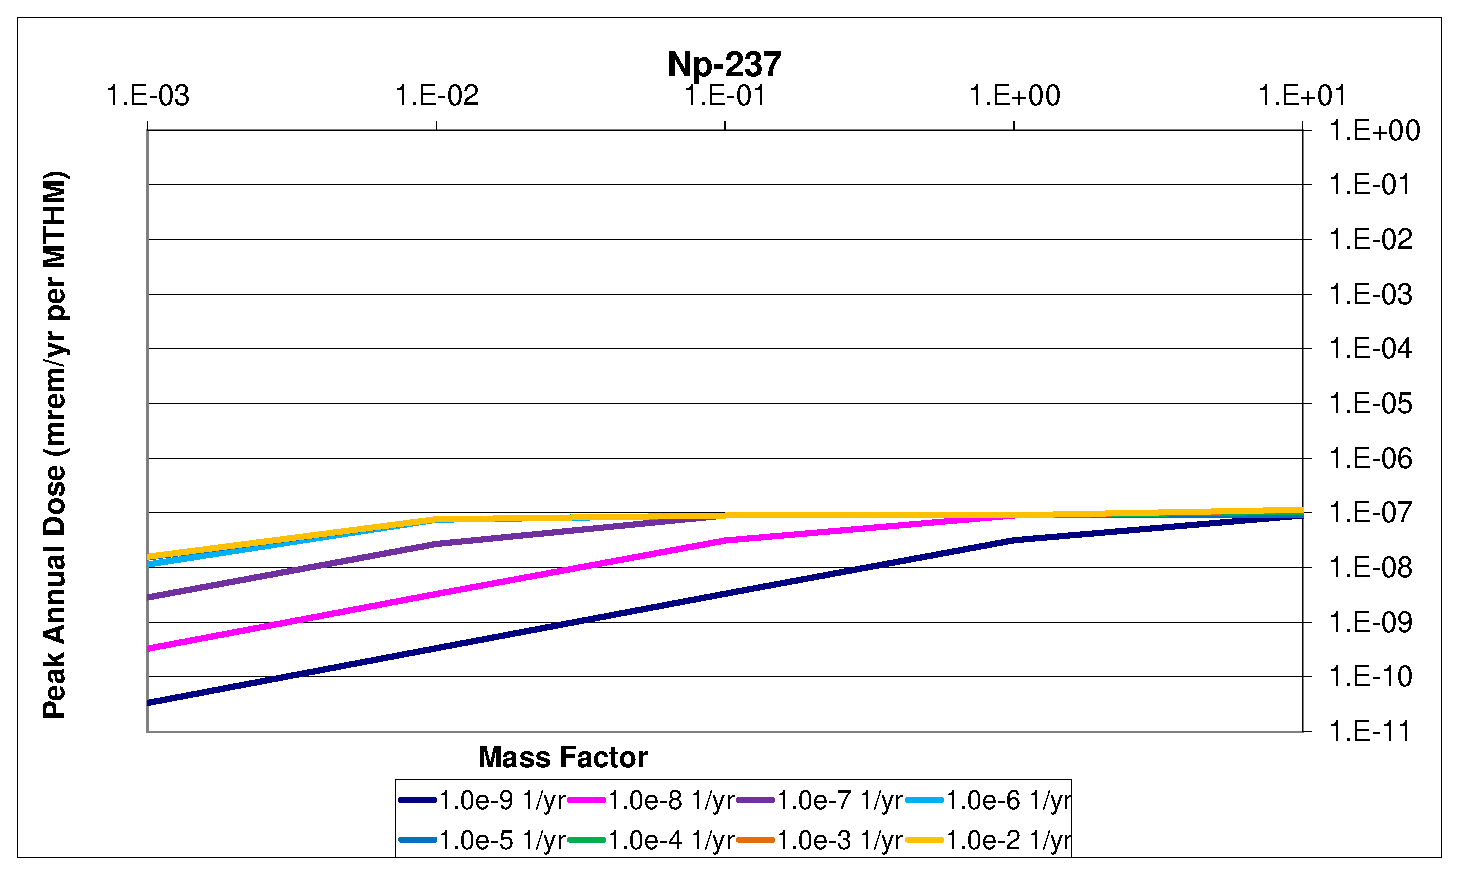
\includegraphics[width=0.8\textwidth]{WFDegAndInv/Np-237-MF.eps}
\caption{
  Solubility limited and sorbing $^{237}Np$ demonstrates a direct proportionality 
to fractional degradation rate until attuation by its solubility limit and other 
natural system parameters. } 
\label{fig:WFDegNp237MF}
\end{figure}

\end{frame}



\subsection{Case VI : Waste Package Failure Time and Diffusion Coefficient}

To investigate the effect of the waste package failure time, it was varied over 
five magnitudes from one thousand to million years. Simultaneously, the reference 
diffusivity was varied over the eight magnitudes between $1\times10^{-8}$ and 
$1\times10^{-15}$ in order to determine the correlation between increased 
radionuclide mobility and the waste package lifetime. 


For the clay repository, the waste package failure time is entirely irrelevant 
until waste package failure times reach the million year time scale. 



\subsection{Vertical Path Length}

Sensitivity of repository performance to characteristics of an advective 
vertical release pathway are examined here.

The model layout assumes that no vertical advective pathway intersects the waste 
packages. Rather, an optional vertical advective pathway with variable length 
can be modeled near the waste packages. This model feature addresses the concern 
that sufficient host medium damage in the evacuation disturbed zone might 
provide a preferred horizontal pathway out of the confines of the repository 
that intersects a fast vertical pathway in which water flows advectively 
upward.

Comparing the effect of the length of the vertical advective path with the 
diffusion coefficent in the \gls{EDZ} and the far field 
provides a notion of the importance of this release pathway. This analysis 
explores the effect of increasing the damage created in evacuation,  
contributes to providing a higher source term at the base of a vertical 
advective pathway. In so doing, this analysis also provides some insight into 
the threshold between primarily diffusive and primarily advective contaminant 
movement. 



\subsection{Parametric Range}

For each value of diffusion coefficient varied in the \gls{EDZ} and far field, 
the vertical path length was varied from 10 to 500 meters.

\begin{table}[ht!]
\centering
\includegraphics[width=0.7\textwidth]{PathLengthAndDiffCoeff/PathLengthAndDiffCoeffGroups.eps}
\caption{Sets of 100 realizations were run for each for vertical advective path 
length and diffusion coefficient coefficient in this dual sensitivity study.}
\label{tab:PathLengthAndDiffCoeffGroups}
\end{table}

\subsection{Results}

This analysis showed that varying advective pathway length within a reasonable 
range had negligible results on repository performance. It also showed that the 
importance of the length of the fast pathway was unaffected by reference 
diffusivities in the \gls{EDZ}. That is, upon changing the reference diffusivity 
in those media simultaneously with the vertical advective pathway length, no 
effect was seen that could be attributed to variability in the advective path 
length. The only variability in the mean of the peak annual doses was due to 
changes in the diffusivity. For this reason it can be concluded that even in the 
case of significant damage to the \gls{EDZ}, the dominant pathway in this 
scenario is the purely diffusive pathway rather than the vertical advective fast 
pathway.



%%%%%%%%%%%%%%%%%%%%%%%%%%%%%%%%%%%%%%%%%%%%%%%%%%%%%%%%%%%%%%%%%%%%%%%%%%%%%%%%
This work is supported by the U.S. Department of Energy, Basic Energy Sciences, 
Office of Nuclear Energy, under con- tract # DE-AC02-06CH11357.



%%%%%%%%%%%%%%%%%%%%%%%%%%%%%%%%%%%%%%%%%%%%%%%%%%%%%%%%%%%%%%%%%%%%%%%%%%%%%%%%
\bibliographystyle{plain}
\bibliography{bibliography}
\end{document}
